\documentclass[twoside]{book}

% Packages required by doxygen
\usepackage{fixltx2e}
\usepackage{calc}
\usepackage{doxygen}
\usepackage[export]{adjustbox} % also loads graphicx
\usepackage{graphicx}
\usepackage[utf8]{inputenc}
\usepackage{makeidx}
\usepackage{multicol}
\usepackage{multirow}
\PassOptionsToPackage{warn}{textcomp}
\usepackage{textcomp}
\usepackage[nointegrals]{wasysym}
\usepackage[table]{xcolor}

% Font selection
\usepackage[T1]{fontenc}
\usepackage[scaled=.90]{helvet}
\usepackage{courier}
\usepackage{amssymb}
\usepackage{sectsty}
\renewcommand{\familydefault}{\sfdefault}
\allsectionsfont{%
  \fontseries{bc}\selectfont%
  \color{darkgray}%
}
\renewcommand{\DoxyLabelFont}{%
  \fontseries{bc}\selectfont%
  \color{darkgray}%
}
\newcommand{\+}{\discretionary{\mbox{\scriptsize$\hookleftarrow$}}{}{}}

% Page & text layout
\usepackage{geometry}
\geometry{%
  a4paper,%
  top=2.5cm,%
  bottom=2.5cm,%
  left=2.5cm,%
  right=2.5cm%
}
\tolerance=750
\hfuzz=15pt
\hbadness=750
\setlength{\emergencystretch}{15pt}
\setlength{\parindent}{0cm}
\setlength{\parskip}{3ex plus 2ex minus 2ex}
\makeatletter
\renewcommand{\paragraph}{%
  \@startsection{paragraph}{4}{0ex}{-1.0ex}{1.0ex}{%
    \normalfont\normalsize\bfseries\SS@parafont%
  }%
}
\renewcommand{\subparagraph}{%
  \@startsection{subparagraph}{5}{0ex}{-1.0ex}{1.0ex}{%
    \normalfont\normalsize\bfseries\SS@subparafont%
  }%
}
\makeatother

% Headers & footers
\usepackage{fancyhdr}
\pagestyle{fancyplain}
\fancyhead[LE]{\fancyplain{}{\bfseries\thepage}}
\fancyhead[CE]{\fancyplain{}{}}
\fancyhead[RE]{\fancyplain{}{\bfseries\leftmark}}
\fancyhead[LO]{\fancyplain{}{\bfseries\rightmark}}
\fancyhead[CO]{\fancyplain{}{}}
\fancyhead[RO]{\fancyplain{}{\bfseries\thepage}}
\fancyfoot[LE]{\fancyplain{}{}}
\fancyfoot[CE]{\fancyplain{}{}}
\fancyfoot[RE]{\fancyplain{}{\bfseries\scriptsize Generated by Doxygen }}
\fancyfoot[LO]{\fancyplain{}{\bfseries\scriptsize Generated by Doxygen }}
\fancyfoot[CO]{\fancyplain{}{}}
\fancyfoot[RO]{\fancyplain{}{}}
\renewcommand{\footrulewidth}{0.4pt}
\renewcommand{\chaptermark}[1]{%
  \markboth{#1}{}%
}
\renewcommand{\sectionmark}[1]{%
  \markright{\thesection\ #1}%
}

% Indices & bibliography
\usepackage{natbib}
\usepackage[titles]{tocloft}
\setcounter{tocdepth}{3}
\setcounter{secnumdepth}{5}
\makeindex

% Packages requested by user
\usepackage{amsmath}

% Hyperlinks (required, but should be loaded last)
\usepackage{ifpdf}
\ifpdf
  \usepackage[pdftex,pagebackref=true]{hyperref}
\else
  \usepackage[ps2pdf,pagebackref=true]{hyperref}
\fi
\hypersetup{%
  colorlinks=true,%
  linkcolor=blue,%
  citecolor=blue,%
  unicode%
}

% Custom commands
\newcommand{\clearemptydoublepage}{%
  \newpage{\pagestyle{empty}\cleardoublepage}%
}

\usepackage{caption}
\captionsetup{labelsep=space,justification=centering,font={bf},singlelinecheck=off,skip=4pt,position=top}

%===== C O N T E N T S =====

\begin{document}

% Titlepage & ToC
\hypersetup{pageanchor=false,
             bookmarksnumbered=true,
             pdfencoding=unicode
            }
\pagenumbering{roman}
\begin{titlepage}
\vspace*{7cm}
\begin{center}%
{\Large Force\+Man\+II \\[1ex]\large 0.\+1 }\\
\vspace*{1cm}
{\large Generated by Doxygen 1.8.11}\\
\end{center}
\end{titlepage}
\clearemptydoublepage
\tableofcontents
\clearemptydoublepage
\pagenumbering{arabic}
\hypersetup{pageanchor=true}

%--- Begin generated contents ---
\chapter{Main Page}
\label{index}\hypertarget{index}{}Welcome to the Force\+Man\+II user/developer manual. This is a work in progress.\hypertarget{index_main_sec}{}\section{Contents}\label{index_main_sec}

\begin{DoxyItemize}
\item Conventions
\begin{DoxyItemize}
\item \hyperlink{terminology}{Terminology}
\item \hyperlink{tinkerformat}{Tinker Force Field Format}
\end{DoxyItemize}
\item Coordinate Types
\begin{DoxyItemize}
\item \hyperlink{distance}{Distance}
\item \hyperlink{angle}{Angle}
\item \hyperlink{torsion}{Torsion}
\end{DoxyItemize}
\item Force Field Terms
\begin{DoxyItemize}
\item \hyperlink{HO}{Harmonic Oscillator}
\item \hyperlink{polynomial}{Polynomial}
\item \hyperlink{fourier}{Fourier Series}
\end{DoxyItemize}
\end{DoxyItemize}\hypertarget{index_Authors}{}\section{Authors}\label{index_Authors}

\begin{DoxyItemize}
\item Original author\+: Ryan M. Richard
\item Additional contributions by\+: No one yet (PR on Git\+Hub to contribute).
\end{DoxyItemize}\hypertarget{index_license_sec}{}\section{License}\label{index_license_sec}
Copyright (C) 2016 Ryan M. Richard $<$ryanmrichard1 at gmail.\+com$>$.

This library is free software; you can redistribute it and/or modify it under the terms of the G\+NU Lesser General Public License as published by the Free Software Foundation; either version 2.\+1 of the License, or (at your option) any later version.

This library is distributed in the hope that it will be useful, but W\+I\+T\+H\+O\+UT A\+NY W\+A\+R\+R\+A\+N\+TY; without even the implied warranty of M\+E\+R\+C\+H\+A\+N\+T\+A\+B\+I\+L\+I\+TY or F\+I\+T\+N\+E\+SS F\+OR A P\+A\+R\+T\+I\+C\+U\+L\+AR P\+U\+R\+P\+O\+SE. See the G\+NU Lesser General Public License for more details.

You should have received a copy of the G\+NU Lesser General Public License along with this library; if not, write to the Free Software Foundation, Inc., 51 Franklin Street, Fifth Floor, Boston, MA 02110-\/1301 U\+SA 
\chapter{Angle Class}
\label{angle}
\hypertarget{angle}{}
The angle class is responsible for normal angle bending terms (i.\+e. those among three bonded atoms). Assuming the vectors $\vec{r_{12}}$ and $\vec{r_{32}}$ are vectors parallel to the bond between atoms 1 and 2 and the bond between atoms 2 and 3 respectively the cosine of the angle between these vectors, $\cos\theta$ is given by\+:

\[ \cos\theta=\frac{\vec{r_{12}}\cdot\vec{r_{32}}} {r_{12} r_{32}}, \] where $r$ denotes the magnitude of $\vec{r}$. We can also express this in terms of the $\sin\theta$\+: \[ \sin\theta=\frac{\left(\vec{r_{12}}\times\vec{r_{32}}\right)\cdot\vec{n}} {r_{12} r_{32} n}, \] where $\frac{\vec{n}}{n}$ is a unit vector perpendicular to both $\vec{r_{12}}$ and $\vec{r_{32}}$. Consequentially, we can also use the tangent of the angle\+: \[ \tan\theta=\frac{\left(\vec{r_{12}}\times\vec{r_{32}}\right)\cdot\vec{n}} {\vec{r_{12}}\cdot\vec{r_{32}}n}. \] 
\chapter{Distance Class}
\label{distance}
\hypertarget{distance}{}
The Distance class is responsible for storing internal coordinates that only depend on the distance between two points in space. This includes\+:
\begin{DoxyItemize}
\item Bond terms
\item Charge-\/charge electrostatic terms
\item Dispersion terms
\item Exchange terms
\end{DoxyItemize}

\subsection*{Mathematical Description}

Given a pair of atoms, the distance $r_{12}$ between them is\+: \[ r_{12}=|\mathbf{r_1}-\mathbf{r_2}|= \sqrt{\sum_{i=1}^3\left(q_{1i}-q_{2i}\right)^2}, \] where $\mathbf{r_i}$ is the position of atom $i$ and $q_{ij}$ is the $j$-\/th Cartesian coordinate of that atom.

The first derivative is\+: \[ \frac{\partial r_{12}}{\partial q_{ij}}=\frac{1}{2r_{12}} \frac{\partial \sum_{k=1}^3\left(q_{1k}-q_{2k}\right)^2}{\partial q_{ij}} =\frac{\pm \left(q_{1j}-q_{2j}\right)}{r_{12}} \] where the plus is for $i=1$ and the minus for $i=2$. 
\chapter{Fourier Series}
\label{fourier}
\hypertarget{fourier}{}
Torsion and improper torsion angles are typically modled as Fourier series. In general a Fourier series has the form\+: \[ E(\theta)=\sum_{n=0}^\infty \frac{1}{2}a_n \cos\left(\frac{2\pi n\theta}{P}-\gamma\right), \] (or a form in which cosine is replaced with sine and the values of the parameters change to reflect that cosine is sine shifted by 90 degrees). Here $P$ is the periodicity of the function, $a_n$ is the height of a particular wave\textquotesingle{}s contribution, and $\gamma$ is a phase shift. In modeling torsions, the angle is periodic every 360 degrees ( $P=2\pi$) and we want the energy to be 0 at the minimum (i.\+e. not -\/1.\+0), hence we usually add 1 to the cosine term, the result is\+: \[ E(\theta)=\sum_{n=0}^\infty \frac{1}{2}a_n\left[1+\cos\left(n\theta-\gamma\right)\right], \] Since most atoms involved in force fields make at most four bonds, the entire potential should be modelable using only the terms up to $n=3$. It is customary to use $\gamma$ so that a minimum occurs at 180 degrees, which means for even $n$, $\gamma=2\pi$ and for odd $n$ $\gamma=0$.

Aside from that the first and second derivatives are easily seen to be\+: \[ \frac{\partial E(\theta)}{\partial \theta}=-\frac{1}{2}\sum_{n=0}^\infty n a_n\sin(n\theta-\gamma) \] and\+: \[ \frac{\partial^2 E(\theta)}{\partial^2 \theta}=-\frac{1}{2}\sum_{n=0}^\infty n^2 a_n\cos(n\theta-\gamma). \]

This pattern continues and we see that the $d$-\/th order derivative is\+: \[ \frac{\partial E(\theta)}{\partial \theta}=(-1)^{(d+1)/2}\frac{1}{2}\sum_{n=0}^\infty n^d a_n\sin(n\theta-\gamma) \] if $d$ is odd, and\+: \[ \frac{\partial^2 E(\theta)}{\partial^2 \theta}=(-1)^{d/2}\frac{1}{2}\sum_{n=0}^\infty n^d a_n\cos(n\theta-\gamma) \] if $d$ is even.

\subsection*{Conventions, i.\+e. What to Do with the Half?}

The Fourier series will ultimately be used for both the torsion and improper torsion angles. Unfortunately, the customary half is not present in the form of the improper torsion. Furthermore, Tinker style parameter files typically bake the half into the torsion parameter already anyways. Unlike the harmonic oscillator where there is actually an advantage to having the half around (it simplifies the derivatives), the half of the Fourier series does nothing for us. For these reasons I have decied to follow Tinker\textquotesingle{}s lead and bake the half into the torsion amplitude parameter.

\subsection*{Implementation Details}

Keeping with the idea of making the interface as simple as possible, the Fourier\+Series class only takes the amplitudes, angles, and periodicities. This is because the derivative only depends on these quantities. The angle is passed in a somewhat special way, namely as $n\theta-\gamma$, this is because this is always the argument to the trig function, regardless of the derivative order. Unlike the harmonic oscillator where we can forget about the details of the shift, for the Fourier series we have to know the value of $n$ for the derivatives. Finally, we ask that for torsions with multiple terms, i.\+e. for torsions that have multiple, and $n,\gamma,a_n$ terms, act as if each set of parameters is a new torsion (call the function once for each set of parameters). 
\chapter{Harmonic Oscillator}
\label{HO}
\hypertarget{HO}{}
One of the cornerstones of physics\textquotesingle{} approximations is the harmonic oscillator. The energy of an $N$-\/dimensional harmonic oscillator is given by\+: \[ E(\vec{q};\vec{k})=\frac{1}{2}\vec{k}\cdot(\vec{q}\circ\vec{q}), \] where $\vec{q}$ is a vector of $N$ coordinates and $\vec{k}$ is a vector of $N$ force constants such that the $q_i$ has force constant $k_i$. $\circ$ denotes the Hadamard product (element-\/wise multiplication), i.\+e. $\left[\vec{q}\circ\vec{q}\right]_{i}=q_i^2$.

The derivative w.\+r.\+t. to $\vec{q}$ is\+: \[ \left[\frac{\partial E(\vec{q};\vec{k})}{\partial\vec{q}}\right]_i=k_i q_i, \] the Hessian is just $\vec{k}$ down the diagonal. All higher derivatives are 0. Doesn\textquotesingle{}t get much easier than that.

\subsection*{Notes on H.\+O. as Implemented in Force\+Man\+II}


\begin{DoxyItemize}
\item As with all force field quantities we assume atomic units are used throughout
\item We explicitly include the 1/2 in our energy formula
\item Usually a H.\+O. measures the energy penelty caused by displacemet from some value $\vec{q_0}$. To simplify the underlying code we assume that input coordinates $\vec{q}=\vec{q}^\prime-\vec{q_0}$ where $\vec{q}^\prime$ is the actual value of the bond, angle, etc. 
\end{DoxyItemize}
\chapter{Polynomial Potential Terms}
\label{polynomial}
\hypertarget{polynomial}{}
Many of the forms of force field potentials are that of polynomials. That is they are a linear combination of $N$ terms of the form\+: \[ E=\sum_{i=1}^Nc_ix^{p_i} \] where $c_i$ is the weight of the $i$-\/th term which has the exponet $p_i$. In general $p_i$ can be positive (say $p_i=2$ for the harmonic oscillator) or negative (say $p_i=-1$ for point-\/charge, point-\/charge interactions). The gradient is\+: \[ \frac{\partial E}{\partial x}=\sum_{i=1}^N c_ip_i x^{p_i-1} \] and the Hessian is\+: \[ \frac{\partial^2 E}{\partial x^2}=\sum_{i=1}^N c_ip_i(P_i-1)x^{p_i-2} \] 
\chapter{Terminology Used Throughout Force\+Man\+II}
\label{terminology}
\hypertarget{terminology}{}
The purpose of this page is to clarify what we mean by some basic terms throughout the manual and throughout the code. I have tried to be consistent but let me know if you find exceptions.


\begin{DoxyItemize}
\item atom number \+: Atoms in an input are listed in some order, whichever atom is listed first is said to have atom number 1, the second is atom number 2, etc.
\item V\+DW type\+: I don\textquotesingle{}t know how standard this is, and I\textquotesingle{}m willing to change the term if someone tells me the standard term for this. Forcefields usually map an atom in a particular chemical enviornment, say an $sp^2$ hybridized carbon in a carbonyl, to a single number, called the V\+DW type. The V\+DW type is then mapped to another number called...
\item atom type\+: This is less specific than the V\+DW type, say all $sp^2$ atoms map to the same atom type. Properties that are more geometric in nature, bonds and angles, tend to list parameters by this type, whereas properties that are more chemical in nature, Coulomb and V\+DW potentials, tend to use the V\+DW type to list parameters. If it helps clarify, atom types are only used internally and are read from the force field, the value you provide to Force\+Man\+II is always the V\+DW type 
\end{DoxyItemize}
\chapter{Tinker Format}
\label{tinkerformat}
\hypertarget{tinkerformat}{}
Finding the actual criteria for the format of the Tiker Parameter file is somewhat difficult so I list it here. The file itself is seperated into three parts. The first part is metadata about the force-\/field such as citations, combining rules, scale factors, etc. The second part lists all recognized atom types and vdw types. The third part lists the parameters arranged by atom or vdw type.

\begin{DoxyNote}{Note}
As implemented in Force\+Man\+II, the Tinker Format is case-\/sensitive
\end{DoxyNote}
\subsection*{Force Field Metadata}

This is the important metadata for a force field\+:


\begin{DoxyItemize}
\item {\ttfamily radiusrule} \+: can be either {\ttfamily A\+R\+I\+T\+H\+M\+E\+T\+IC} or {\ttfamily G\+E\+O\+M\+E\+T\+R\+IC}. This is the type of the average used to combine the van Der Waals radii
\item {\ttfamily radiussize} \+: is the radius a {\ttfamily R\+A\+D\+I\+US} or a {\ttfamily D\+I\+A\+M\+E\+T\+ER}
\item {\ttfamily epsilonrul} \+: same as {\ttfamily radiusrule} except for the well-\/depth
\item {\ttfamily vdw-\/14-\/scale} \+: this is a scale factor that will be applied to the van Der Waals interactions between 1-\/4 bonded atoms, i.\+e. ends of a torsion angle
\item {\ttfamily chg-\/14-\/scale} \+: same as {\ttfamily vdw-\/14-\/scale} except for the charges
\item {\ttfamily electric} \+: the electric perm 332.\+0522173
\item {\ttfamily dielectric} \+: the dielectric constant (or absolute permitivity) for the force field in the same units as the electric permetivity
\end{DoxyItemize}

\subsection*{Atom Types and V\+DW Types}

This is the specification of the atom and vdw types the format is\+:


\begin{DoxyCode}
1 atom <vdw type> <atom type> <symbol> <description> <atomic number> <mass> <number of bonds
\end{DoxyCode}



\begin{DoxyItemize}
\item {\ttfamily atom} \+: this is flag to specify that we are defining vdw and atom types
\item {\ttfamily vdw type} \+: this is an integer specifying which vdw type we are defnining
\item {\ttfamily atom type} \+: this is an integer specifying the atom type
\item {\ttfamily symobl} \+: 1 to 2 characters for the atom type, is usually some mixture of the atomic symbol and a letter to describe the chemical environment like T for terminal
\item {\ttfamily description} \+: a string giving a more readable description
\item {\ttfamily atomic number} \+: The atomic number of the atom as it appears on the periodic table
\item {\ttfamily mass} \+: the isotope averaged mass of the atom in Daltons, i.\+e. the mass you find on the periodic table
\item {\ttfamily number of bonds} \+: the usual number of bonds that an atom of this vdw type makes
\end{DoxyItemize}

\subsection*{Parameters}

The order of the parameter sections does not matter aside from the fact that if a parameter occurs more than once, i.\+e. you specify the force constant for atom types 1 and 2 twice, the last value will be used.

\subsubsection*{Harmonic Bond Stretching Potential}


\begin{DoxyCode}
1 bond   <atom type 1>  <atom type 2> <force constant> <r\_0>
\end{DoxyCode}



\begin{DoxyItemize}
\item {\ttfamily bond} \+: a flag to specify these parameters are for bonds
\item {\ttfamily atom type 1} \+: the atom type of one of the two atoms
\item {\ttfamily atom type 2} \+: the atom type for the other atom
\item {\ttfamily force constant} \+: the force constant in kcal/(mol Angstrom$^\wedge$2), the 1/2 of the harmonic potential is included
\item {\ttfamily r\+\_\+0} \+: the equilibrium distance for the bond in Angstroms
\end{DoxyItemize}

\subsubsection*{Angle-\/\+Bending Harmonic Potential Parameters}


\begin{DoxyCode}
1 angle  <atom type 1> <vertex atom type> <atom type 2> <force constant> <theta\_0>
\end{DoxyCode}



\begin{DoxyItemize}
\item {\ttfamily angle} \+: a flag to specify that these are parameters for an angle
\item {\ttfamily atom type 1} \+: one of the non-\/vertex atoms\textquotesingle{} types
\item {\ttfamily vertex atom type} \+: the atom type of the vertex atom
\item {\ttfamily atom type 2} \+: the other non-\/vertex atom\textquotesingle{}s type
\item {\ttfamily force constant} \+: the force constant in kcal/(mol$\ast$radians$^\wedge$2)
\item {\ttfamily theta\+\_\+0} \+: the equilibrium angle in degrees
\end{DoxyItemize}

\#\#\# Torsion Fourier-\/\+Series Parameters 
\begin{DoxyCode}
1 torsion <end 1> <center 1> <center 2> <end 2> <V> <gamma> <n> [<V> <gamma> <n> [<V> <gamma> <n>]] 
\end{DoxyCode}



\begin{DoxyItemize}
\item {\ttfamily torsion} \+: a flag specifying these are parameters for a proper torsion
\item {\ttfamily end 1} \+: the atom type of one of the ends of the torsion angle
\item {\ttfamily center 1} \+: the atom type of the central atom bonded to the first end atom
\item {\ttfamily center 2} \+: the atom type of the next central atom
\item {\ttfamily end 2} \+: the atom type of the other end atom
\item {\ttfamily V} \+: the amplitude of the Fourier Series component in kcal/mol
\item {\ttfamily gamma} \+: the equlibrium value of the torsion in degrees
\item {\ttfamily n} \+: the periodicity of the Fourier Series component
\item Other values of {\ttfamily V}, {\ttfamily gamma}, and {\ttfamily n} can optionally be repeated up to another two times to specify additional terms in the Fourier Series for this interaction
\end{DoxyItemize}

\#\#\# Improper Torsion Fourier-\/\+Series Parameters 
\begin{DoxyCode}
1 imptors <atom type 1> <atom type 2> <central atom type> <atom type 3> <V> <gamma> <n>
\end{DoxyCode}



\begin{DoxyItemize}
\item {\ttfamily imptors} \+: a flag specifying these are parameters for an improper torsion
\item {\ttfamily atom type 1} \+: the atom type of one of the orbital atoms
\item {\ttfamily atom type 2} \+: the atom type of one of the other orbital atoms
\item {\ttfamily central atom type} \+: the atom type of the central atom
\item {\ttfamily atom type 3} \+: the atom type of the last orbital atom
\item {\ttfamily V} \+: the amplitude of the Fourier Series component in kcal/mol
\item {\ttfamily gamma} \+: the equlibrium value of the torsion in degrees
\item {\ttfamily n} \+: the periodicity of the Fourier Series component
\end{DoxyItemize}

\subsubsection*{Charge-\/\+Charge Potential Parameters}


\begin{DoxyCode}
1 charge <vdw type> <q>
\end{DoxyCode}



\begin{DoxyItemize}
\item {\ttfamily charge} \+: a flag specifying these parameters are for a charge
\item {\ttfamily vdw type} \+: the vdw type of the atom
\item {\ttfamily q} \+: the charge in atomic units, i.\+e. number of electrons
\end{DoxyItemize}

\subsubsection*{Lennard-\/\+Jones 6-\/12 Potential Parameters}


\begin{DoxyCode}
1 vdw           <atom\_type>               <radius> <epsilon>
\end{DoxyCode}



\begin{DoxyItemize}
\item {\ttfamily vdw} \+: a flag to specify that these are parameters for van Der Waals interaction
\item {\ttfamily atom\+\_\+type} \+: the atom type this parameter is for
\item {\ttfamily radius} \+: the radius (or diameter depending on the metadata provided) in Angstroms
\item {\ttfamily epsilon} \+: the well depth in kcal/mol 
\end{DoxyItemize}
\chapter{Torsion Angle Class}
\label{torsion}
\hypertarget{torsion}{}
\begin{DoxyWarning}{Warning}
Energies computed by Forceman\+II for the torsional and improper torsional energetic components may differ from those of other programs. Read on to see why this is.
\end{DoxyWarning}
\section*{Torsion}

Assume that atom 1 is bonded to atom 2; atom 2 is bonded to atom3, and atom 3 is bonded to atom 4. If we look down the 2-\/3 bond the 1-\/2 and 2-\/3 bonds will make an angle. This angle is the torsion angle. Mathematically this can be viewed as the angle between plane comprised of atoms 1,2, and 3 and the plane comprised of the atoms 2,3,4. Let $\vec{r_{21}}$ be a vector parallel to the 1-\/2 bond pointing from atom 2 to atom 1, $\vec{r_{23}}$ be a vector parallel to the 2-\/3 bond pointing from atom 2 to atom 3, and $\vec{r_{34}}$ be a vector parallel to the 3-\/4 bond pointing from atom 3 to atom 4. $\vec{n_1}=\vec{r_{21}}\times\vec{r_{23}}$ is a vector normal to the plane containing atoms 1, 2, and 3 and $\vec{n_2}=\vec{r_{34}}\times\vec{r_{23}}$ is a vector normal to the plane containing atoms 2, 3, and 4. The dihedral angle, $\phi$ is then given by\+: \[ \cos\theta=\frac{\vec{n_1}\cdot\vec{n_2}}{n_1 n_2}. \] Alternatively\+: \[ \vec{n_1}\times\vec{n_2}=\frac{n_1 n_2\sin\theta \vec{n_3}}{n_3} \] where $\vec{n_3}$ is a unit vector perpindicular to $\vec{n_1}$ and $\vec{n_2}$ and with direction consistent with the right-\/hand rule. Since, both of our cross products involved $\vec{r_{23}}$, we know that $\vec{n_3}=\frac{\vec{r_{23}}}{r_{23}}$. Given that $\vec{n_3}$ is a unit vector we may multiply both sides of the previous equation from the right by it to get\+: \[ \sin\theta=\frac{\left(\vec{n_1}\times\vec{n_2}\right)\cdot\vec{r_{23}}} {n_1 n_2 r_{23}} \] Using the fact that $\tan\theta=\frac{\sin\theta}{\cos\theta}$ we also have \[ \tan\theta=\frac{\left(\vec{n_1}\times\vec{n_2}\right)\cdot\vec{r_{23}}} {r_{23}} \]

As far as symmetries of the torsion angle are concerned, we have one degree of freedom, we can read the sequence forward or backward. Presently, we choose to read the sequence in which ever manner makes atoms 2 and atoms 3 show up in number order (order in input). Parameters for torsions are expected to be given in an analogous manner (atom type 2 should be less then atom type 3).

\subsection*{Improper Torsion}

Related to the torsion angle, the improper torsion angle measures the planarity around an sp $^2$ hybridized atom. Instead of being a non-\/branching path i.\+e. 1 is connected to 2, which is connected to 3, which is connected to 4, the atoms in an improper torsion are all bonded to atom 2. It should be noted that there are other conventions for which atom the central atom is (usually that it is atom 3), but we choose it to be atom 2 as this is naturally where it falls when looping over connectivity.

It is also worth noting a few properties of the improper dihedral angle. Assume for a quadruple of atoms \$ a\+\_\+1,a\+\_\+2,a\+\_\+3,a\+\_\+4\$, we always compute our dihedral angle as the angle between the planes formed from the first three atoms, $a_1, a_2, a_3$, and the last three atoms, $a_2, a_3, a_4$. If we swap the atom originally labeled as 2 and the atom originally labeled as 3, which is the differing conventions for where the central atom goes, the angle changes sign. Swapping atom 1 and atom 4 produces the same sign change. However, swapping atoms 1 and 3 produces a different angle than the original, and swapping 3 and 4 produces yet another unique angle. This is a problem as there are three unique angles that can be generated just by interchanging the order in which the atoms are numbered. After a long search, the best information I can find is on \href{http://chempedia.info/info/165388/}{\tt this website}. Basically they suggest that the order of the orbtial atoms is that of their input and the central atom is given third for A\+M\+B\+ER and first for C\+H\+A\+R\+MM. Again, our code requests that the central atom is given second.

In order to ensure we always compute the same angle, regardless of the order in which the atoms are specified in the input file, we compute the torsions based on the atom type; specifically, the atom that has the lowest atom type is the first atom, atom two is always the central atom, atom 3 is the atom with the next lowest atom type, and atom 4 is the atom with the highest atom type. In the event of a tie, we number the atoms with the same atom types in a clockwise fashion around the central atom. This is most easily done by computing the angle between the vector going from the central atom to the unique atom and the vector going from the central atom to the non-\/unique atom. Lowest angle is closest to the unique angle in a clockwise sense 
\chapter{Namespace Index}
\section{Namespace List}
Here is a list of all documented namespaces with brief descriptions\+:\begin{DoxyCompactList}
\item\contentsline{section}{\hyperlink{namespaceFManII}{F\+Man\+II} \\*Namespace for all code associated with Force\+Man\+II }{\pageref{namespaceFManII}}{}
\end{DoxyCompactList}

\chapter{Hierarchical Index}
\section{Class Hierarchy}
This inheritance list is sorted roughly, but not completely, alphabetically\+:\begin{DoxyCompactList}
\item \contentsline{section}{F\+Man\+II\+:\+:F\+F\+Term$<$ Model\+\_\+t, Coord\+\_\+t $>$}{\pageref{classFManII_1_1FFTerm}}{}
\item \contentsline{section}{F\+Man\+II\+:\+:Fourier\+Series}{\pageref{structFManII_1_1FourierSeries}}{}
\item \contentsline{section}{F\+Man\+II\+:\+:Harmonic\+Oscillator}{\pageref{structFManII_1_1HarmonicOscillator}}{}
\item \contentsline{section}{F\+Man\+II\+:\+:Int\+Coords}{\pageref{classFManII_1_1IntCoords}}{}
\begin{DoxyCompactList}
\item \contentsline{section}{F\+Man\+II\+:\+:Angle}{\pageref{classFManII_1_1Angle}}{}
\item \contentsline{section}{F\+Man\+II\+:\+:Distance}{\pageref{classFManII_1_1Distance}}{}
\item \contentsline{section}{F\+Man\+II\+:\+:Torsion}{\pageref{classFManII_1_1Torsion}}{}
\end{DoxyCompactList}
\end{DoxyCompactList}

\chapter{Class Index}
\section{Class List}
Here are the classes, structs, unions and interfaces with brief descriptions\+:\begin{DoxyCompactList}
\item\contentsline{section}{\hyperlink{classFManII_1_1Angle}{F\+Man\+I\+I\+::\+Angle} }{\pageref{classFManII_1_1Angle}}{}
\item\contentsline{section}{\hyperlink{classFManII_1_1Distance}{F\+Man\+I\+I\+::\+Distance} }{\pageref{classFManII_1_1Distance}}{}
\item\contentsline{section}{\hyperlink{classFManII_1_1FFTerm}{F\+Man\+I\+I\+::\+F\+F\+Term$<$ Model\+\_\+t, Coord\+\_\+t $>$} }{\pageref{classFManII_1_1FFTerm}}{}
\item\contentsline{section}{\hyperlink{structFManII_1_1FourierSeries}{F\+Man\+I\+I\+::\+Fourier\+Series} \\*Implements a Fourier Series model potential }{\pageref{structFManII_1_1FourierSeries}}{}
\item\contentsline{section}{\hyperlink{structFManII_1_1HarmonicOscillator}{F\+Man\+I\+I\+::\+Harmonic\+Oscillator} \\*Implements the harmonic oscillator model potential }{\pageref{structFManII_1_1HarmonicOscillator}}{}
\item\contentsline{section}{\hyperlink{classFManII_1_1IntCoords}{F\+Man\+I\+I\+::\+Int\+Coords} \\*A base class designed to provide basic functionality to things like bonds, angles, etc }{\pageref{classFManII_1_1IntCoords}}{}
\item\contentsline{section}{\hyperlink{classFManII_1_1Torsion}{F\+Man\+I\+I\+::\+Torsion} }{\pageref{classFManII_1_1Torsion}}{}
\end{DoxyCompactList}

\chapter{File Index}
\section{File List}
Here is a list of all documented files with brief descriptions\+:\begin{DoxyCompactList}
\item\contentsline{section}{\hyperlink{Angle_8hpp}{Angle.\+hpp} }{\pageref{Angle_8hpp}}{}
\item\contentsline{section}{\hyperlink{Common_8hpp}{Common.\+hpp} }{\pageref{Common_8hpp}}{}
\item\contentsline{section}{\hyperlink{Distance_8hpp}{Distance.\+hpp} }{\pageref{Distance_8hpp}}{}
\item\contentsline{section}{\hyperlink{FFTerm_8hpp}{F\+F\+Term.\+hpp} }{\pageref{FFTerm_8hpp}}{}
\item\contentsline{section}{\hyperlink{FManII_8hpp}{F\+Man\+I\+I.\+hpp} \\*This header is meant to be the main A\+PI to Force\+Man\+II. Anything users need to interface with Force\+Man\+II goes here }{\pageref{FManII_8hpp}}{}
\item\contentsline{section}{\hyperlink{FourierSeries_8hpp}{Fourier\+Series.\+hpp} }{\pageref{FourierSeries_8hpp}}{}
\item\contentsline{section}{\hyperlink{HarmonicOscillator_8hpp}{Harmonic\+Oscillator.\+hpp} }{\pageref{HarmonicOscillator_8hpp}}{}
\item\contentsline{section}{{\bfseries Internal\+Coordinates.\+hpp} }{\pageref{InternalCoordinates_8hpp}}{}
\item\contentsline{section}{\hyperlink{Torsion_8hpp}{Torsion.\+hpp} }{\pageref{Torsion_8hpp}}{}
\item\contentsline{section}{\hyperlink{Util_8hpp}{Util.\+hpp} }{\pageref{Util_8hpp}}{}
\end{DoxyCompactList}

\chapter{Namespace Documentation}
\hypertarget{namespaceFManII}{}\section{F\+Man\+II Namespace Reference}
\label{namespaceFManII}\index{F\+Man\+II@{F\+Man\+II}}


Namespace for all code associated with Force\+Man\+II.  


\subsection*{Classes}
\begin{DoxyCompactItemize}
\item 
class \hyperlink{classFManII_1_1Angle}{Angle}
\item 
class \hyperlink{classFManII_1_1Distance}{Distance}
\item 
class \hyperlink{classFManII_1_1FFTerm}{F\+F\+Term}
\item 
struct \hyperlink{structFManII_1_1FourierSeries}{Fourier\+Series}
\begin{DoxyCompactList}\small\item\em Implements a Fourier Series model potential. \end{DoxyCompactList}\item 
struct \hyperlink{structFManII_1_1HarmonicOscillator}{Harmonic\+Oscillator}
\begin{DoxyCompactList}\small\item\em Implements the harmonic oscillator model potential. \end{DoxyCompactList}\item 
class \hyperlink{classFManII_1_1IntCoords}{Int\+Coords}
\begin{DoxyCompactList}\small\item\em A base class designed to provide basic functionality to things like bonds, angles, etc. \end{DoxyCompactList}\item 
class \hyperlink{classFManII_1_1Torsion}{Torsion}
\end{DoxyCompactItemize}
\subsection*{Typedefs}
\begin{DoxyCompactItemize}
\item 
using {\bfseries D\+Vector} = std\+::vector$<$ double $>$\hypertarget{namespaceFManII_a7f89f8915272399dda44b281ae39a94a}{}\label{namespaceFManII_a7f89f8915272399dda44b281ae39a94a}

\item 
using {\bfseries I\+Vector} = std\+::vector$<$ size\+\_\+t $>$\hypertarget{namespaceFManII_a314ed8350c41700525e12966212980e9}{}\label{namespaceFManII_a314ed8350c41700525e12966212980e9}

\item 
{\footnotesize template$<$size\+\_\+t n$>$ }\\using {\bfseries I\+Array} = std\+::array$<$ size\+\_\+t, \hyperlink{namespaceFManII_ab331802fde4c5f2564443f1704c25363a351f38f2149aa0e3be56f7c5aa16eae9}{n} $>$\hypertarget{namespaceFManII_a8360f8defc13d25e7131179fcd33ffd2}{}\label{namespaceFManII_a8360f8defc13d25e7131179fcd33ffd2}

\item 
using {\bfseries shared\+\_\+\+D\+Vector} = std\+::shared\+\_\+ptr$<$ const D\+Vector $>$\hypertarget{namespaceFManII_ab3ad101443820b6b8a263fdccb2aaae3}{}\label{namespaceFManII_ab3ad101443820b6b8a263fdccb2aaae3}

\item 
using {\bfseries D\+Array} = std\+::array$<$ double, 3 $>$\hypertarget{namespaceFManII_af7bb56e0807edff7d188ff037a09d35f}{}\label{namespaceFManII_af7bb56e0807edff7d188ff037a09d35f}

\item 
using \hyperlink{namespaceFManII_a988516dba14437f483faf9f3c6d40c25}{Coord\+Array} = std\+::map$<$ \hyperlink{namespaceFManII_aee2b0c5668a8970ffb58ac650994e059}{Int\+Coord\+\_\+t}, std\+::unique\+\_\+ptr$<$ \hyperlink{classFManII_1_1IntCoords}{Int\+Coords} $>$$>$\hypertarget{namespaceFManII_a988516dba14437f483faf9f3c6d40c25}{}\label{namespaceFManII_a988516dba14437f483faf9f3c6d40c25}

\begin{DoxyCompactList}\small\item\em An array of internal coordinates arranged by type. \end{DoxyCompactList}\item 
using \hyperlink{namespaceFManII_add1cccdf9425a71de6835b2631b84db8}{Atom\+Types} = std\+::vector$<$ std\+::array$<$ size\+\_\+t, 2 $>$$>$\hypertarget{namespaceFManII_add1cccdf9425a71de6835b2631b84db8}{}\label{namespaceFManII_add1cccdf9425a71de6835b2631b84db8}

\begin{DoxyCompactList}\small\item\em Array where element i respectively is the atom type and V\+DW type of atom i. \end{DoxyCompactList}\item 
using \hyperlink{namespaceFManII_a7c18a61f01fcc0604c39cbfae43665df}{Conn\+Data} = std\+::vector$<$ std\+::vector$<$ size\+\_\+t $>$$>$\hypertarget{namespaceFManII_a7c18a61f01fcc0604c39cbfae43665df}{}\label{namespaceFManII_a7c18a61f01fcc0604c39cbfae43665df}

\begin{DoxyCompactList}\small\item\em Array such that element i is a vector of the atoms bonded to atom i. \end{DoxyCompactList}\item 
using \hyperlink{namespaceFManII_a16edca665b5dfcdf9b3995844ad01bb5}{Param\+Types} = std\+::map$<$ \hyperlink{namespaceFManII_aee2b0c5668a8970ffb58ac650994e059}{Int\+Coord\+\_\+t}, std\+::map$<$ \hyperlink{namespaceFManII_ab331802fde4c5f2564443f1704c25363}{Param\+\_\+t}, std\+::map$<$ std\+::vector$<$ size\+\_\+t $>$, double $>$$>$$>$
\begin{DoxyCompactList}\small\item\em An object to hold the parameters of a force field. \end{DoxyCompactList}\end{DoxyCompactItemize}
\subsection*{Enumerations}
\begin{DoxyCompactItemize}
\item 
enum \hyperlink{namespaceFManII_ab331802fde4c5f2564443f1704c25363}{Param\+\_\+t} \{ \\*
\hyperlink{namespaceFManII_ab331802fde4c5f2564443f1704c25363acce4c4e3a7008d8a210e0950f0ae6646}{K}, 
\hyperlink{namespaceFManII_ab331802fde4c5f2564443f1704c25363adbd624e837d07235c15569341fa0c052}{r0}, 
\hyperlink{namespaceFManII_ab331802fde4c5f2564443f1704c25363a807f5303050e210f41b43189457ee216}{amp}, 
\hyperlink{namespaceFManII_ab331802fde4c5f2564443f1704c25363a3a18cc339dcc327297994fd5de406000}{phi}, 
\\*
\hyperlink{namespaceFManII_ab331802fde4c5f2564443f1704c25363a351f38f2149aa0e3be56f7c5aa16eae9}{n}, 
\hyperlink{namespaceFManII_ab331802fde4c5f2564443f1704c25363a6168b053bb4d250bc56878c3c5329606}{amp2}, 
\hyperlink{namespaceFManII_ab331802fde4c5f2564443f1704c25363ac923a156e5d6c899b0691bcf05dbfe08}{phi2}, 
\hyperlink{namespaceFManII_ab331802fde4c5f2564443f1704c25363a79574f7c7d028868bba201ab99eeb319}{n2}, 
\\*
\hyperlink{namespaceFManII_ab331802fde4c5f2564443f1704c25363a8ea674fa14845cb499bba588e8e6b72d}{amp3}, 
\hyperlink{namespaceFManII_ab331802fde4c5f2564443f1704c25363a48029f18757fa6d2a3d72517001cc0d1}{phi3}, 
\hyperlink{namespaceFManII_ab331802fde4c5f2564443f1704c25363ac582c34207ea213912ced08cebca1a34}{n3}, 
\hyperlink{namespaceFManII_ab331802fde4c5f2564443f1704c25363afec764e5c20f480b9b706861106356de}{q}, 
\\*
\hyperlink{namespaceFManII_ab331802fde4c5f2564443f1704c25363a0cdd92becbae953906c5305392e29836}{sigma}, 
\hyperlink{namespaceFManII_ab331802fde4c5f2564443f1704c25363a59874bb4d679327306f2c7405286afa9}{epsilon}
 \}\begin{DoxyCompactList}\small\item\em These are the recognized types of parameters. \end{DoxyCompactList}
\item 
enum \hyperlink{namespaceFManII_aee2b0c5668a8970ffb58ac650994e059}{Int\+Coord\+\_\+t} \{ \\*
\hyperlink{namespaceFManII_aee2b0c5668a8970ffb58ac650994e059a0ad48919334546233ad86a2699918852}{B\+O\+ND}, 
\hyperlink{namespaceFManII_aee2b0c5668a8970ffb58ac650994e059ae3fda21c728a90c9974bb2a2404efcc7}{U\+B\+P\+A\+IR}, 
\hyperlink{namespaceFManII_aee2b0c5668a8970ffb58ac650994e059ad387432e20772e11fb6520606b93faa6}{P\+A\+IR}, 
\hyperlink{namespaceFManII_aee2b0c5668a8970ffb58ac650994e059ad67623636070f3be7ae6e7700a5bd9f6}{A\+N\+G\+LE}, 
\\*
\hyperlink{namespaceFManII_aee2b0c5668a8970ffb58ac650994e059a4f481d454dea70e1a1c7ef63d99d3402}{T\+O\+R\+S\+I\+ON}, 
\hyperlink{namespaceFManII_aee2b0c5668a8970ffb58ac650994e059a650ab62f01654d8aae5b3a9c9919dbed}{I\+M\+P\+T\+O\+R\+S\+I\+ON}, 
\hyperlink{namespaceFManII_aee2b0c5668a8970ffb58ac650994e059af32be9c7ba6cd66722cc93629dbb5fbe}{E\+L\+E\+C\+T\+R\+O\+S\+T\+A\+T\+I\+CS}, 
\hyperlink{namespaceFManII_aee2b0c5668a8970ffb58ac650994e059a97b415b3364dd5c1da0fd17a551ce037}{L\+E\+N\+N\+A\+R\+D\+\_\+\+J\+O\+N\+ES}
 \}\begin{DoxyCompactList}\small\item\em These are the recognized types of Int\+Coords. \end{DoxyCompactList}
\end{DoxyCompactItemize}
\subsection*{Functions}
\begin{DoxyCompactItemize}
\item 
V\+Double {\bfseries angle} (const double $\ast$r1, const double $\ast$r2, const double $\ast$r3, double off)\hypertarget{namespaceFManII_ac145eebe2971f15a0053dbd0926c7b9a}{}\label{namespaceFManII_ac145eebe2971f15a0053dbd0926c7b9a}

\item 
{\footnotesize template$<$typename T , typename... Args$>$ }\\std\+::unique\+\_\+ptr$<$ T $>$ \hyperlink{namespaceFManII_a57e9a715666f24e78bd0025020e2c08e}{make\+\_\+unique} (Args \&\&...args)\hypertarget{namespaceFManII_a57e9a715666f24e78bd0025020e2c08e}{}\label{namespaceFManII_a57e9a715666f24e78bd0025020e2c08e}

\begin{DoxyCompactList}\small\item\em Once C++14 is accepted we can use std\+::make\+\_\+unique, till then we have this. \end{DoxyCompactList}\item 
void {\bfseries C\+H\+E\+CK} (bool cond, const std\+::string \&msg)\hypertarget{namespaceFManII_a70d1cfbb2f83f24521e0f0a31df25fd4}{}\label{namespaceFManII_a70d1cfbb2f83f24521e0f0a31df25fd4}

\item 
std\+::vector$<$ double $>$ {\bfseries dist} (const double $\ast$q1, const double $\ast$q2, double off)\hypertarget{namespaceFManII_a7570392168766203fc6452d09cad01cf}{}\label{namespaceFManII_a7570392168766203fc6452d09cad01cf}

\item 
void {\bfseries add\+\_\+bond} (const I\+Vector \&Atoms, const \hyperlink{namespaceFManII_add1cccdf9425a71de6835b2631b84db8}{Atom\+Types} \&Types, const \hyperlink{namespaceFManII_a16edca665b5dfcdf9b3995844ad01bb5}{Param\+Types} \&Params, \hyperlink{namespaceFManII_a988516dba14437f483faf9f3c6d40c25}{Coord\+Array} \&Found\+Coords)\hypertarget{namespaceFManII_a3218348ba8f97811883d92317dcfea94}{}\label{namespaceFManII_a3218348ba8f97811883d92317dcfea94}

\item 
void {\bfseries add\+\_\+angle} (const I\+Vector \&Atoms, const \hyperlink{namespaceFManII_add1cccdf9425a71de6835b2631b84db8}{Atom\+Types} \&Types, const \hyperlink{namespaceFManII_a16edca665b5dfcdf9b3995844ad01bb5}{Param\+Types} \&Params, \hyperlink{namespaceFManII_a988516dba14437f483faf9f3c6d40c25}{Coord\+Array} \&Found\+Coords)\hypertarget{namespaceFManII_a2d03d3143239d96b6ab10e2d1c56af66}{}\label{namespaceFManII_a2d03d3143239d96b6ab10e2d1c56af66}

\item 
void {\bfseries add\+\_\+torsion} (const I\+Vector \&Atoms, const \hyperlink{namespaceFManII_add1cccdf9425a71de6835b2631b84db8}{Atom\+Types} \&Types, const \hyperlink{namespaceFManII_a16edca665b5dfcdf9b3995844ad01bb5}{Param\+Types} \&Params, \hyperlink{namespaceFManII_a988516dba14437f483faf9f3c6d40c25}{Coord\+Array} \&Found\+Coords)\hypertarget{namespaceFManII_a881ebfcaac60e0da1409cc566861ab52}{}\label{namespaceFManII_a881ebfcaac60e0da1409cc566861ab52}

\item 
void {\bfseries add\+\_\+imp} (const I\+Vector \&Atoms, const \hyperlink{namespaceFManII_add1cccdf9425a71de6835b2631b84db8}{Atom\+Types} \&Types, const \hyperlink{namespaceFManII_a16edca665b5dfcdf9b3995844ad01bb5}{Param\+Types} \&Params, \hyperlink{namespaceFManII_a988516dba14437f483faf9f3c6d40c25}{Coord\+Array} \&Found\+Coords, const D\+Vector \&carts)\hypertarget{namespaceFManII_a3ebe80f5c7bbe67ecd94fd2512858045}{}\label{namespaceFManII_a3ebe80f5c7bbe67ecd94fd2512858045}

\item 
void {\bfseries add\+\_\+electrostatics} (const I\+Vector \&Atoms, const \hyperlink{namespaceFManII_add1cccdf9425a71de6835b2631b84db8}{Atom\+Types} \&Types, const \hyperlink{namespaceFManII_a16edca665b5dfcdf9b3995844ad01bb5}{Param\+Types} \&Params, \hyperlink{namespaceFManII_a988516dba14437f483faf9f3c6d40c25}{Coord\+Array} \&Found\+Coords, const D\+Vector \&carts)\hypertarget{namespaceFManII_a8e4be217fb18b91403f97d99b3b4c8ac}{}\label{namespaceFManII_a8e4be217fb18b91403f97d99b3b4c8ac}

\item 
\hyperlink{namespaceFManII_a988516dba14437f483faf9f3c6d40c25}{Coord\+Array} \hyperlink{namespaceFManII_a962553cf7a05889bf0f90071a59d963c}{get\+\_\+coords} (const std\+::vector$<$ double $>$ \&Carts, const \hyperlink{namespaceFManII_add1cccdf9425a71de6835b2631b84db8}{Atom\+Types} \&Types, const \hyperlink{namespaceFManII_a16edca665b5dfcdf9b3995844ad01bb5}{Param\+Types} \&Params, const \hyperlink{namespaceFManII_a7c18a61f01fcc0604c39cbfae43665df}{Conn\+Data} \&Conns, double chg14scale=1.\+0)
\begin{DoxyCompactList}\small\item\em A function that processes the input and returns a set of objects set up for use in \hyperlink{namespaceFManII}{F\+Man\+II}. \end{DoxyCompactList}\item 
void {\bfseries add\+\_\+eletrostatics} (const I\+Vector \&Atoms, const A\+Tom\+Types \&Types, \hyperlink{namespaceFManII_a988516dba14437f483faf9f3c6d40c25}{Coord\+Array} \&Found\+Coords, double scale)\hypertarget{namespaceFManII_a7cd24ffeba90b8bfc9e235e550021d75}{}\label{namespaceFManII_a7cd24ffeba90b8bfc9e235e550021d75}

\item 
{\footnotesize template$<$typename T , typename T2 , typename T3 $>$ }\\I\+Array$<$ 3 $>$ {\bfseries order\+\_\+imp} (size\+\_\+t common, size\+\_\+t v1, size\+\_\+t v2, const T \&spokes, const T2 \&mags, const T3 \&ts)\hypertarget{namespaceFManII_abbb76098dc0ce293eb77c39ea451ecec}{}\label{namespaceFManII_abbb76098dc0ce293eb77c39ea451ecec}

\item 
double {\bfseries odd\+\_\+deriv\+\_\+} (size\+\_\+t d, double Q, double V, double \hyperlink{namespaceFManII_ab331802fde4c5f2564443f1704c25363a351f38f2149aa0e3be56f7c5aa16eae9}{n})\hypertarget{namespaceFManII_a4d1c3cdc99779ef25b59ec9bce04bc3f}{}\label{namespaceFManII_a4d1c3cdc99779ef25b59ec9bce04bc3f}

\item 
double {\bfseries even\+\_\+deriv\+\_\+} (size\+\_\+t d, double Q, double V, double \hyperlink{namespaceFManII_ab331802fde4c5f2564443f1704c25363a351f38f2149aa0e3be56f7c5aa16eae9}{n})\hypertarget{namespaceFManII_a15ad94b985d81cac64aaca5c84f8d06e}{}\label{namespaceFManII_a15ad94b985d81cac64aaca5c84f8d06e}

\item 
Deriv\+\_\+t {\bfseries torsion} (const double $\ast$q1, const double $\ast$q2, const double $\ast$q3, const double $\ast$q4, double \hyperlink{namespaceFManII_ab331802fde4c5f2564443f1704c25363a351f38f2149aa0e3be56f7c5aa16eae9}{n}, double gamma)\hypertarget{namespaceFManII_a4d60b97475fdf4736295110c685e1f8b}{}\label{namespaceFManII_a4d60b97475fdf4736295110c685e1f8b}

\item 
{\footnotesize template$<$typename T $>$ }\\std\+::array$<$ double, 3 $>$ \hyperlink{namespaceFManII_ab6c3ba0221d1479590c328071add3a69}{cross} (const T \&v1, const T \&v2)\hypertarget{namespaceFManII_ab6c3ba0221d1479590c328071add3a69}{}\label{namespaceFManII_ab6c3ba0221d1479590c328071add3a69}

\begin{DoxyCompactList}\small\item\em Returns the cross product of two vectors. \end{DoxyCompactList}\item 
{\footnotesize template$<$typename T $>$ }\\std\+::array$<$ double, 3 $>$ \hyperlink{namespaceFManII_a67d2288b51cdc78b0569812bbbe7603c}{diff} (const T \&v1, const T \&v2)\hypertarget{namespaceFManII_a67d2288b51cdc78b0569812bbbe7603c}{}\label{namespaceFManII_a67d2288b51cdc78b0569812bbbe7603c}

\begin{DoxyCompactList}\small\item\em Returns the difference between two vectors, v1-\/v2. \end{DoxyCompactList}\item 
double \hyperlink{namespaceFManII_a804811720c4566ddd330e4abc8d2c65f}{dot} (const std\+::array$<$ double, 3 $>$ \&v1, const std\+::array$<$ double, 3 $>$ \&v2)\hypertarget{namespaceFManII_a804811720c4566ddd330e4abc8d2c65f}{}\label{namespaceFManII_a804811720c4566ddd330e4abc8d2c65f}

\begin{DoxyCompactList}\small\item\em Returns the dot product of two vectors. \end{DoxyCompactList}\item 
double \hyperlink{namespaceFManII_a88126c99fc2140b9a3c37d695337fd6a}{mag} (const std\+::array$<$ double, 3 $>$ \&v1)\hypertarget{namespaceFManII_a88126c99fc2140b9a3c37d695337fd6a}{}\label{namespaceFManII_a88126c99fc2140b9a3c37d695337fd6a}

\begin{DoxyCompactList}\small\item\em Returns the magnitude of a vector. \end{DoxyCompactList}\item 
double \hyperlink{namespaceFManII_a45ace6891d8e67f7e4b679300533e0ac}{angle} (const std\+::array$<$ double, 3 $>$ \&v1, const std\+::array$<$ double, 3 $>$ \&v2, const std\+::array$<$ double, 3 $>$ \&\hyperlink{namespaceFManII_ab331802fde4c5f2564443f1704c25363a351f38f2149aa0e3be56f7c5aa16eae9}{n})
\end{DoxyCompactItemize}


\subsection{Typedef Documentation}
\index{F\+Man\+II@{F\+Man\+II}!Param\+Types@{Param\+Types}}
\index{Param\+Types@{Param\+Types}!F\+Man\+II@{F\+Man\+II}}
\subsubsection[{\texorpdfstring{Param\+Types}{ParamTypes}}]{\setlength{\rightskip}{0pt plus 5cm}using {\bf F\+Man\+I\+I\+::\+Param\+Types} = typedef std\+::map$<${\bf Int\+Coord\+\_\+t},std\+::map$<${\bf Param\+\_\+t}, std\+::map$<$std\+::vector$<$size\+\_\+t$>$,double$>$$>$$>$}\hypertarget{namespaceFManII_a16edca665b5dfcdf9b3995844ad01bb5}{}\label{namespaceFManII_a16edca665b5dfcdf9b3995844ad01bb5}
If you like you can think of this as a rank 3 tensor. The first rank tells us which of the recognized internal coordinates the parameters are for. The second rank tells us which of the recognized types of parameters the set is and the third rank tells us the atom type. Putting that all together, the bond force constant between say atoms of type 3 and 4 is given by\+: 
\begin{DoxyCode}
\hyperlink{namespaceFManII_a16edca665b5dfcdf9b3995844ad01bb5}{ParamTypes} params;\textcolor{comment}{//Assume we already had this}
\textcolor{keywordtype}{double} k=params[FManII::Bond][\hyperlink{namespaceFManII_ab331802fde4c5f2564443f1704c25363acce4c4e3a7008d8a210e0950f0ae6646}{FManII::K}][\{3,4\}];
\end{DoxyCode}
 

\subsection{Enumeration Type Documentation}
\index{F\+Man\+II@{F\+Man\+II}!Int\+Coord\+\_\+t@{Int\+Coord\+\_\+t}}
\index{Int\+Coord\+\_\+t@{Int\+Coord\+\_\+t}!F\+Man\+II@{F\+Man\+II}}
\subsubsection[{\texorpdfstring{Int\+Coord\+\_\+t}{IntCoord_t}}]{\setlength{\rightskip}{0pt plus 5cm}enum {\bf F\+Man\+I\+I\+::\+Int\+Coord\+\_\+t}}\hypertarget{namespaceFManII_aee2b0c5668a8970ffb58ac650994e059}{}\label{namespaceFManII_aee2b0c5668a8970ffb58ac650994e059}
\begin{Desc}
\item[Enumerator]\par
\begin{description}
\index{B\+O\+ND@{B\+O\+ND}!F\+Man\+II@{F\+Man\+II}}\index{F\+Man\+II@{F\+Man\+II}!B\+O\+ND@{B\+O\+ND}}\item[{\em 
B\+O\+ND\hypertarget{namespaceFManII_aee2b0c5668a8970ffb58ac650994e059a0ad48919334546233ad86a2699918852}{}\label{namespaceFManII_aee2b0c5668a8970ffb58ac650994e059a0ad48919334546233ad86a2699918852}
}]A bond. \index{U\+B\+P\+A\+IR@{U\+B\+P\+A\+IR}!F\+Man\+II@{F\+Man\+II}}\index{F\+Man\+II@{F\+Man\+II}!U\+B\+P\+A\+IR@{U\+B\+P\+A\+IR}}\item[{\em 
U\+B\+P\+A\+IR\hypertarget{namespaceFManII_aee2b0c5668a8970ffb58ac650994e059ae3fda21c728a90c9974bb2a2404efcc7}{}\label{namespaceFManII_aee2b0c5668a8970ffb58ac650994e059ae3fda21c728a90c9974bb2a2404efcc7}
}]A 1,3 pair. \index{P\+A\+IR@{P\+A\+IR}!F\+Man\+II@{F\+Man\+II}}\index{F\+Man\+II@{F\+Man\+II}!P\+A\+IR@{P\+A\+IR}}\item[{\em 
P\+A\+IR\hypertarget{namespaceFManII_aee2b0c5668a8970ffb58ac650994e059ad387432e20772e11fb6520606b93faa6}{}\label{namespaceFManII_aee2b0c5668a8970ffb58ac650994e059ad387432e20772e11fb6520606b93faa6}
}]A pair that is not a bond or a 1,3 pair. \index{A\+N\+G\+LE@{A\+N\+G\+LE}!F\+Man\+II@{F\+Man\+II}}\index{F\+Man\+II@{F\+Man\+II}!A\+N\+G\+LE@{A\+N\+G\+LE}}\item[{\em 
A\+N\+G\+LE\hypertarget{namespaceFManII_aee2b0c5668a8970ffb58ac650994e059ad67623636070f3be7ae6e7700a5bd9f6}{}\label{namespaceFManII_aee2b0c5668a8970ffb58ac650994e059ad67623636070f3be7ae6e7700a5bd9f6}
}]An angle. \index{T\+O\+R\+S\+I\+ON@{T\+O\+R\+S\+I\+ON}!F\+Man\+II@{F\+Man\+II}}\index{F\+Man\+II@{F\+Man\+II}!T\+O\+R\+S\+I\+ON@{T\+O\+R\+S\+I\+ON}}\item[{\em 
T\+O\+R\+S\+I\+ON\hypertarget{namespaceFManII_aee2b0c5668a8970ffb58ac650994e059a4f481d454dea70e1a1c7ef63d99d3402}{}\label{namespaceFManII_aee2b0c5668a8970ffb58ac650994e059a4f481d454dea70e1a1c7ef63d99d3402}
}]A torsion. \index{I\+M\+P\+T\+O\+R\+S\+I\+ON@{I\+M\+P\+T\+O\+R\+S\+I\+ON}!F\+Man\+II@{F\+Man\+II}}\index{F\+Man\+II@{F\+Man\+II}!I\+M\+P\+T\+O\+R\+S\+I\+ON@{I\+M\+P\+T\+O\+R\+S\+I\+ON}}\item[{\em 
I\+M\+P\+T\+O\+R\+S\+I\+ON\hypertarget{namespaceFManII_aee2b0c5668a8970ffb58ac650994e059a650ab62f01654d8aae5b3a9c9919dbed}{}\label{namespaceFManII_aee2b0c5668a8970ffb58ac650994e059a650ab62f01654d8aae5b3a9c9919dbed}
}]An improper torsion angle. \index{E\+L\+E\+C\+T\+R\+O\+S\+T\+A\+T\+I\+CS@{E\+L\+E\+C\+T\+R\+O\+S\+T\+A\+T\+I\+CS}!F\+Man\+II@{F\+Man\+II}}\index{F\+Man\+II@{F\+Man\+II}!E\+L\+E\+C\+T\+R\+O\+S\+T\+A\+T\+I\+CS@{E\+L\+E\+C\+T\+R\+O\+S\+T\+A\+T\+I\+CS}}\item[{\em 
E\+L\+E\+C\+T\+R\+O\+S\+T\+A\+T\+I\+CS\hypertarget{namespaceFManII_aee2b0c5668a8970ffb58ac650994e059af32be9c7ba6cd66722cc93629dbb5fbe}{}\label{namespaceFManII_aee2b0c5668a8970ffb58ac650994e059af32be9c7ba6cd66722cc93629dbb5fbe}
}]A charge-\/charge interaction. \index{L\+E\+N\+N\+A\+R\+D\+\_\+\+J\+O\+N\+ES@{L\+E\+N\+N\+A\+R\+D\+\_\+\+J\+O\+N\+ES}!F\+Man\+II@{F\+Man\+II}}\index{F\+Man\+II@{F\+Man\+II}!L\+E\+N\+N\+A\+R\+D\+\_\+\+J\+O\+N\+ES@{L\+E\+N\+N\+A\+R\+D\+\_\+\+J\+O\+N\+ES}}\item[{\em 
L\+E\+N\+N\+A\+R\+D\+\_\+\+J\+O\+N\+ES\hypertarget{namespaceFManII_aee2b0c5668a8970ffb58ac650994e059a97b415b3364dd5c1da0fd17a551ce037}{}\label{namespaceFManII_aee2b0c5668a8970ffb58ac650994e059a97b415b3364dd5c1da0fd17a551ce037}
}]A 6-\/12 Lennard-\/\+Jones potential. \end{description}
\end{Desc}
\index{F\+Man\+II@{F\+Man\+II}!Param\+\_\+t@{Param\+\_\+t}}
\index{Param\+\_\+t@{Param\+\_\+t}!F\+Man\+II@{F\+Man\+II}}
\subsubsection[{\texorpdfstring{Param\+\_\+t}{Param_t}}]{\setlength{\rightskip}{0pt plus 5cm}enum {\bf F\+Man\+I\+I\+::\+Param\+\_\+t}}\hypertarget{namespaceFManII_ab331802fde4c5f2564443f1704c25363}{}\label{namespaceFManII_ab331802fde4c5f2564443f1704c25363}
\begin{Desc}
\item[Enumerator]\par
\begin{description}
\index{K@{K}!F\+Man\+II@{F\+Man\+II}}\index{F\+Man\+II@{F\+Man\+II}!K@{K}}\item[{\em 
K\hypertarget{namespaceFManII_ab331802fde4c5f2564443f1704c25363acce4c4e3a7008d8a210e0950f0ae6646}{}\label{namespaceFManII_ab331802fde4c5f2564443f1704c25363acce4c4e3a7008d8a210e0950f0ae6646}
}]A force constant. \index{r0@{r0}!F\+Man\+II@{F\+Man\+II}}\index{F\+Man\+II@{F\+Man\+II}!r0@{r0}}\item[{\em 
r0\hypertarget{namespaceFManII_ab331802fde4c5f2564443f1704c25363adbd624e837d07235c15569341fa0c052}{}\label{namespaceFManII_ab331802fde4c5f2564443f1704c25363adbd624e837d07235c15569341fa0c052}
}]The equilibrium value. \index{amp@{amp}!F\+Man\+II@{F\+Man\+II}}\index{F\+Man\+II@{F\+Man\+II}!amp@{amp}}\item[{\em 
amp\hypertarget{namespaceFManII_ab331802fde4c5f2564443f1704c25363a807f5303050e210f41b43189457ee216}{}\label{namespaceFManII_ab331802fde4c5f2564443f1704c25363a807f5303050e210f41b43189457ee216}
}]The amplitude for Fourier series. \index{phi@{phi}!F\+Man\+II@{F\+Man\+II}}\index{F\+Man\+II@{F\+Man\+II}!phi@{phi}}\item[{\em 
phi\hypertarget{namespaceFManII_ab331802fde4c5f2564443f1704c25363a3a18cc339dcc327297994fd5de406000}{}\label{namespaceFManII_ab331802fde4c5f2564443f1704c25363a3a18cc339dcc327297994fd5de406000}
}]The phase shift for Fourier series. \index{n@{n}!F\+Man\+II@{F\+Man\+II}}\index{F\+Man\+II@{F\+Man\+II}!n@{n}}\item[{\em 
n\hypertarget{namespaceFManII_ab331802fde4c5f2564443f1704c25363a351f38f2149aa0e3be56f7c5aa16eae9}{}\label{namespaceFManII_ab331802fde4c5f2564443f1704c25363a351f38f2149aa0e3be56f7c5aa16eae9}
}]The periodicity for Fourier series. \index{amp2@{amp2}!F\+Man\+II@{F\+Man\+II}}\index{F\+Man\+II@{F\+Man\+II}!amp2@{amp2}}\item[{\em 
amp2\hypertarget{namespaceFManII_ab331802fde4c5f2564443f1704c25363a6168b053bb4d250bc56878c3c5329606}{}\label{namespaceFManII_ab331802fde4c5f2564443f1704c25363a6168b053bb4d250bc56878c3c5329606}
}]The amplitude for a two-\/part Fourier series. \index{phi2@{phi2}!F\+Man\+II@{F\+Man\+II}}\index{F\+Man\+II@{F\+Man\+II}!phi2@{phi2}}\item[{\em 
phi2\hypertarget{namespaceFManII_ab331802fde4c5f2564443f1704c25363ac923a156e5d6c899b0691bcf05dbfe08}{}\label{namespaceFManII_ab331802fde4c5f2564443f1704c25363ac923a156e5d6c899b0691bcf05dbfe08}
}]The phase shift for a two-\/part Fourier series. \index{n2@{n2}!F\+Man\+II@{F\+Man\+II}}\index{F\+Man\+II@{F\+Man\+II}!n2@{n2}}\item[{\em 
n2\hypertarget{namespaceFManII_ab331802fde4c5f2564443f1704c25363a79574f7c7d028868bba201ab99eeb319}{}\label{namespaceFManII_ab331802fde4c5f2564443f1704c25363a79574f7c7d028868bba201ab99eeb319}
}]The periodicity for a two-\/part Fourier series. \index{amp3@{amp3}!F\+Man\+II@{F\+Man\+II}}\index{F\+Man\+II@{F\+Man\+II}!amp3@{amp3}}\item[{\em 
amp3\hypertarget{namespaceFManII_ab331802fde4c5f2564443f1704c25363a8ea674fa14845cb499bba588e8e6b72d}{}\label{namespaceFManII_ab331802fde4c5f2564443f1704c25363a8ea674fa14845cb499bba588e8e6b72d}
}]The amplitude for a three-\/part Fourier series. \index{phi3@{phi3}!F\+Man\+II@{F\+Man\+II}}\index{F\+Man\+II@{F\+Man\+II}!phi3@{phi3}}\item[{\em 
phi3\hypertarget{namespaceFManII_ab331802fde4c5f2564443f1704c25363a48029f18757fa6d2a3d72517001cc0d1}{}\label{namespaceFManII_ab331802fde4c5f2564443f1704c25363a48029f18757fa6d2a3d72517001cc0d1}
}]The phase shift for a three-\/part Fourier series. \index{n3@{n3}!F\+Man\+II@{F\+Man\+II}}\index{F\+Man\+II@{F\+Man\+II}!n3@{n3}}\item[{\em 
n3\hypertarget{namespaceFManII_ab331802fde4c5f2564443f1704c25363ac582c34207ea213912ced08cebca1a34}{}\label{namespaceFManII_ab331802fde4c5f2564443f1704c25363ac582c34207ea213912ced08cebca1a34}
}]The periodicity for a three-\/part Fourier series. \index{q@{q}!F\+Man\+II@{F\+Man\+II}}\index{F\+Man\+II@{F\+Man\+II}!q@{q}}\item[{\em 
q\hypertarget{namespaceFManII_ab331802fde4c5f2564443f1704c25363afec764e5c20f480b9b706861106356de}{}\label{namespaceFManII_ab331802fde4c5f2564443f1704c25363afec764e5c20f480b9b706861106356de}
}]The charge, in a.\+u., for point-\/charge, point-\/charge. \index{sigma@{sigma}!F\+Man\+II@{F\+Man\+II}}\index{F\+Man\+II@{F\+Man\+II}!sigma@{sigma}}\item[{\em 
sigma\hypertarget{namespaceFManII_ab331802fde4c5f2564443f1704c25363a0cdd92becbae953906c5305392e29836}{}\label{namespaceFManII_ab331802fde4c5f2564443f1704c25363a0cdd92becbae953906c5305392e29836}
}]The radius of a 6-\/12 potential. \index{epsilon@{epsilon}!F\+Man\+II@{F\+Man\+II}}\index{F\+Man\+II@{F\+Man\+II}!epsilon@{epsilon}}\item[{\em 
epsilon\hypertarget{namespaceFManII_ab331802fde4c5f2564443f1704c25363a59874bb4d679327306f2c7405286afa9}{}\label{namespaceFManII_ab331802fde4c5f2564443f1704c25363a59874bb4d679327306f2c7405286afa9}
}]The well depth of a 6-\/12 potential. \end{description}
\end{Desc}


\subsection{Function Documentation}
\index{F\+Man\+II@{F\+Man\+II}!angle@{angle}}
\index{angle@{angle}!F\+Man\+II@{F\+Man\+II}}
\subsubsection[{\texorpdfstring{angle(const std\+::array$<$ double, 3 $>$ \&v1, const std\+::array$<$ double, 3 $>$ \&v2, const std\+::array$<$ double, 3 $>$ \&n)}{angle(const std::array< double, 3 > &v1, const std::array< double, 3 > &v2, const std::array< double, 3 > &n)}}]{\setlength{\rightskip}{0pt plus 5cm}double F\+Man\+I\+I\+::angle (
\begin{DoxyParamCaption}
\item[{const std\+::array$<$ double, 3 $>$ \&}]{v1, }
\item[{const std\+::array$<$ double, 3 $>$ \&}]{v2, }
\item[{const std\+::array$<$ double, 3 $>$ \&}]{n}
\end{DoxyParamCaption}
)\hspace{0.3cm}{\ttfamily [inline]}}\hypertarget{namespaceFManII_a45ace6891d8e67f7e4b679300533e0ac}{}\label{namespaceFManII_a45ace6891d8e67f7e4b679300533e0ac}
Returns the angle between two vectors given the vectors {\ttfamily v1}, {\ttfamily v2} and a normal to them {\ttfamily n} (vectors need not be units already) \index{F\+Man\+II@{F\+Man\+II}!get\+\_\+coords@{get\+\_\+coords}}
\index{get\+\_\+coords@{get\+\_\+coords}!F\+Man\+II@{F\+Man\+II}}
\subsubsection[{\texorpdfstring{get\+\_\+coords(const std\+::vector$<$ double $>$ \&\+Carts, const Atom\+Types \&\+Types, const Param\+Types \&\+Params, const Conn\+Data \&\+Conns, double chg14scale=1.\+0)}{get_coords(const std::vector< double > &Carts, const AtomTypes &Types, const ParamTypes &Params, const ConnData &Conns, double chg14scale=1.0)}}]{\setlength{\rightskip}{0pt plus 5cm}{\bf Coord\+Array} F\+Man\+I\+I\+::get\+\_\+coords (
\begin{DoxyParamCaption}
\item[{const std\+::vector$<$ double $>$ \&}]{Carts, }
\item[{const {\bf Atom\+Types} \&}]{Types, }
\item[{const {\bf Param\+Types} \&}]{Params, }
\item[{const {\bf Conn\+Data} \&}]{Conns, }
\item[{double}]{chg14scale = {\ttfamily 1.0}}
\end{DoxyParamCaption}
)}\hypertarget{namespaceFManII_a962553cf7a05889bf0f90071a59d963c}{}\label{namespaceFManII_a962553cf7a05889bf0f90071a59d963c}
See the documentation for each type for information on how to set it up. Each type is actually just a typedef of S\+TL containers so no other resources of \hyperlink{namespaceFManII}{F\+Man\+II} are needed to run this function.


\begin{DoxyParams}[1]{Parameters}
\mbox{\tt in}  & {\em Carts} & The Cartesian coordinates in a.\+u. of each atom in the form $x,y,z$ of atom 1, then $x,y,z$ of atom 2, etc. \\
\hline
\mbox{\tt in}  & {\em Types} & An array of the atom types of each atom \\
\hline
\mbox{\tt in}  & {\em Params} & The parameters for the force field \\
\hline
\mbox{\tt in}  & {\em Conns} & The connectivity information \\
\hline
\mbox{\tt in}  & {\em chg14scale} & How much should 1-\/4 electrostatics be scaled by \\
\hline
\end{DoxyParams}

\chapter{Class Documentation}
\hypertarget{classFManII_1_1Angle}{}\section{F\+Man\+II\+:\+:Angle Class Reference}
\label{classFManII_1_1Angle}\index{F\+Man\+I\+I\+::\+Angle@{F\+Man\+I\+I\+::\+Angle}}


{\ttfamily \#include $<$Angle.\+hpp$>$}



Inheritance diagram for F\+Man\+II\+:\+:Angle\+:\nopagebreak
\begin{figure}[H]
\begin{center}
\leavevmode
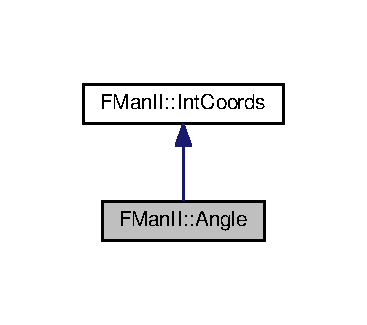
\includegraphics[width=176pt]{classFManII_1_1Angle__inherit__graph}
\end{center}
\end{figure}


Collaboration diagram for F\+Man\+II\+:\+:Angle\+:\nopagebreak
\begin{figure}[H]
\begin{center}
\leavevmode
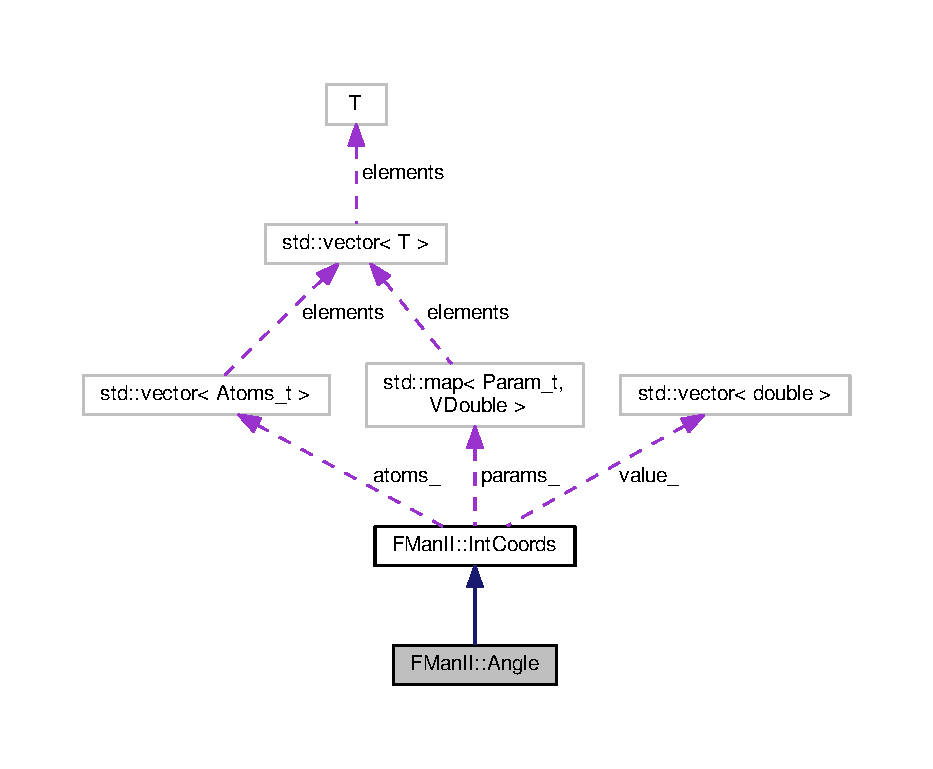
\includegraphics[width=350pt]{classFManII_1_1Angle__coll__graph}
\end{center}
\end{figure}
\subsection*{Public Member Functions}
\begin{DoxyCompactItemize}
\item 
{\bfseries Angle} (std\+::shared\+\_\+ptr$<$ const \hyperlink{classFManII_1_1IntCoords_af42df2795dec16350f908cfd5ac2ef06}{V\+Double} $>$ Carts)\hypertarget{classFManII_1_1Angle_af4d80ba2399fd3b569c427ab2afba0ad}{}\label{classFManII_1_1Angle_af4d80ba2399fd3b569c427ab2afba0ad}

\item 
{\footnotesize template$<$typename... args$>$ }\\void \hyperlink{classFManII_1_1IntCoords_aaa13717daa2c47a00c56e8dcb18896b6}{add\+\_\+coord} (const \hyperlink{classFManII_1_1IntCoords_a59ab25571f774fca97644a2ce5ade359}{Atoms\+\_\+t} \&coord, \hyperlink{namespaceFManII_ab331802fde4c5f2564443f1704c25363}{Param\+\_\+t} param, double pvalue, args...\+other\+\_\+params)
\begin{DoxyCompactList}\small\item\em The call to add a coordinate to this Int\+Coord. \end{DoxyCompactList}\item 
const \hyperlink{classFManII_1_1IntCoords_af42df2795dec16350f908cfd5ac2ef06}{V\+Double} \& \hyperlink{classFManII_1_1IntCoords_a8b36508bebeb262d2c41bed1301ad9f9}{values} () const \hypertarget{classFManII_1_1IntCoords_a8b36508bebeb262d2c41bed1301ad9f9}{}\label{classFManII_1_1IntCoords_a8b36508bebeb262d2c41bed1301ad9f9}

\begin{DoxyCompactList}\small\item\em Returns the array of coordinates. \end{DoxyCompactList}\item 
const \hyperlink{classFManII_1_1IntCoords_af42df2795dec16350f908cfd5ac2ef06}{V\+Double} \& \hyperlink{classFManII_1_1IntCoords_ac107ad541179d838052f37538883671a}{params} (\hyperlink{namespaceFManII_ab331802fde4c5f2564443f1704c25363}{Param\+\_\+t} pt) const \hypertarget{classFManII_1_1IntCoords_ac107ad541179d838052f37538883671a}{}\label{classFManII_1_1IntCoords_ac107ad541179d838052f37538883671a}

\begin{DoxyCompactList}\small\item\em Returns the array of a particular parameter. \end{DoxyCompactList}\end{DoxyCompactItemize}
\subsection*{Protected Types}
\begin{DoxyCompactItemize}
\item 
using \hyperlink{classFManII_1_1IntCoords_a59ab25571f774fca97644a2ce5ade359}{Atoms\+\_\+t} = std\+::vector$<$ size\+\_\+t $>$\hypertarget{classFManII_1_1IntCoords_a59ab25571f774fca97644a2ce5ade359}{}\label{classFManII_1_1IntCoords_a59ab25571f774fca97644a2ce5ade359}

\begin{DoxyCompactList}\small\item\em Typedef for the set of atoms in an Int\+Coord. \end{DoxyCompactList}\item 
using \hyperlink{classFManII_1_1IntCoords_af42df2795dec16350f908cfd5ac2ef06}{V\+Double} = std\+::vector$<$ double $>$\hypertarget{classFManII_1_1IntCoords_af42df2795dec16350f908cfd5ac2ef06}{}\label{classFManII_1_1IntCoords_af42df2795dec16350f908cfd5ac2ef06}

\begin{DoxyCompactList}\small\item\em Typedef for a vector of doubles. \end{DoxyCompactList}\end{DoxyCompactItemize}
\subsection*{Protected Member Functions}
\begin{DoxyCompactItemize}
\item 
\hyperlink{classFManII_1_1IntCoords_af42df2795dec16350f908cfd5ac2ef06}{V\+Double} \hyperlink{classFManII_1_1Angle_a48105b9c14048db6ccea1a410e8943f1}{compute\+\_\+value} (size\+\_\+t deriv\+\_\+i, \hyperlink{classFManII_1_1IntCoords_a59ab25571f774fca97644a2ce5ade359}{Atoms\+\_\+t} coord\+\_\+i) const 
\begin{DoxyCompactList}\small\item\em Overridden by the derived class so that it computes the i-\/th derivative of the coordinate which involves the specified atoms. \end{DoxyCompactList}\item 
void \hyperlink{classFManII_1_1IntCoords_a21ae6c2eb4a0dbea71a402f399061d5b}{add\+\_\+coord} (const \hyperlink{classFManII_1_1IntCoords_a59ab25571f774fca97644a2ce5ade359}{Atoms\+\_\+t} \&coord)\hypertarget{classFManII_1_1IntCoords_a21ae6c2eb4a0dbea71a402f399061d5b}{}\label{classFManII_1_1IntCoords_a21ae6c2eb4a0dbea71a402f399061d5b}

\begin{DoxyCompactList}\small\item\em Recursion end point. \end{DoxyCompactList}\end{DoxyCompactItemize}
\subsection*{Protected Attributes}
\begin{DoxyCompactItemize}
\item 
size\+\_\+t \hyperlink{classFManII_1_1IntCoords_a3fb097438609927dda0f1a049ff61a72}{natoms\+\_\+}\hypertarget{classFManII_1_1IntCoords_a3fb097438609927dda0f1a049ff61a72}{}\label{classFManII_1_1IntCoords_a3fb097438609927dda0f1a049ff61a72}

\begin{DoxyCompactList}\small\item\em The number of atoms this coordinate depends on. \end{DoxyCompactList}\item 
std\+::shared\+\_\+ptr$<$ const \hyperlink{classFManII_1_1IntCoords_af42df2795dec16350f908cfd5ac2ef06}{V\+Double} $>$ \hyperlink{classFManII_1_1IntCoords_a54cd82d40213e7c85ea338b79438b22a}{carts\+\_\+}\hypertarget{classFManII_1_1IntCoords_a54cd82d40213e7c85ea338b79438b22a}{}\label{classFManII_1_1IntCoords_a54cd82d40213e7c85ea338b79438b22a}

\begin{DoxyCompactList}\small\item\em The cartesian coordinates of the system in a.\+u. \end{DoxyCompactList}\item 
\hyperlink{classFManII_1_1IntCoords_af42df2795dec16350f908cfd5ac2ef06}{V\+Double} \hyperlink{classFManII_1_1IntCoords_a1dfc726f1b6060c0f4e26eafb51953f9}{value\+\_\+}\hypertarget{classFManII_1_1IntCoords_a1dfc726f1b6060c0f4e26eafb51953f9}{}\label{classFManII_1_1IntCoords_a1dfc726f1b6060c0f4e26eafb51953f9}

\begin{DoxyCompactList}\small\item\em The actual length of the bond, or angle of the angle, etc. \end{DoxyCompactList}\item 
std\+::vector$<$ \hyperlink{classFManII_1_1IntCoords_a59ab25571f774fca97644a2ce5ade359}{Atoms\+\_\+t} $>$ \hyperlink{classFManII_1_1IntCoords_a4f7c142879fb222c66ae6968160d36c0}{atoms\+\_\+}\hypertarget{classFManII_1_1IntCoords_a4f7c142879fb222c66ae6968160d36c0}{}\label{classFManII_1_1IntCoords_a4f7c142879fb222c66ae6968160d36c0}

\begin{DoxyCompactList}\small\item\em The atom numbers associated with each value. \end{DoxyCompactList}\item 
std\+::map$<$ \hyperlink{namespaceFManII_ab331802fde4c5f2564443f1704c25363}{Param\+\_\+t}, \hyperlink{classFManII_1_1IntCoords_af42df2795dec16350f908cfd5ac2ef06}{V\+Double} $>$ \hyperlink{classFManII_1_1IntCoords_ab1a5fd9c10badbeb02ac40516a7183cc}{params\+\_\+}\hypertarget{classFManII_1_1IntCoords_ab1a5fd9c10badbeb02ac40516a7183cc}{}\label{classFManII_1_1IntCoords_ab1a5fd9c10badbeb02ac40516a7183cc}

\begin{DoxyCompactList}\small\item\em The parameters associated with this set of internal coordinates. \end{DoxyCompactList}\end{DoxyCompactItemize}


\subsection{Detailed Description}
Implements derivatives for angle among three points. See \hyperlink{angle}{Angle Class} for more detail. 

\subsection{Member Function Documentation}
\index{F\+Man\+I\+I\+::\+Angle@{F\+Man\+I\+I\+::\+Angle}!add\+\_\+coord@{add\+\_\+coord}}
\index{add\+\_\+coord@{add\+\_\+coord}!F\+Man\+I\+I\+::\+Angle@{F\+Man\+I\+I\+::\+Angle}}
\subsubsection[{\texorpdfstring{add\+\_\+coord(const Atoms\+\_\+t \&coord, Param\+\_\+t param, double pvalue, args...\+other\+\_\+params)}{add_coord(const Atoms_t &coord, Param_t param, double pvalue, args...other_params)}}]{\setlength{\rightskip}{0pt plus 5cm}template$<$typename... args$>$ void F\+Man\+I\+I\+::\+Int\+Coords\+::add\+\_\+coord (
\begin{DoxyParamCaption}
\item[{const {\bf Atoms\+\_\+t} \&}]{coord, }
\item[{{\bf Param\+\_\+t}}]{param, }
\item[{double}]{pvalue, }
\item[{args...}]{other\+\_\+params}
\end{DoxyParamCaption}
)\hspace{0.3cm}{\ttfamily [inline]}, {\ttfamily [inherited]}}\hypertarget{classFManII_1_1IntCoords_aaa13717daa2c47a00c56e8dcb18896b6}{}\label{classFManII_1_1IntCoords_aaa13717daa2c47a00c56e8dcb18896b6}
Don\textquotesingle{}t be offput by the signature using this function is pretty easy. The first argument is the atoms in this coordinate. The remaining 2N arguments are the N parameters associated with this coordinate. They must be in the order parameter type, value of that parameter, next parameter type, value of the next parameter, etc. You will get a compile time error if you do not supply pairs for each parameter or if you mix up the order.

Point is usage looks like this\+: 
\begin{DoxyCode}
\textcolor{comment}{//Assume these are already made instances of IntCoords}
\hyperlink{classFManII_1_1IntCoords_aff5b80e7f579dd8aeac5200942b4db87}{IntCoords} MyBonds,MyAngles;

\textcolor{comment}{//Adds a bond between atoms 1 and 2 with a force constant of 3.4}
MyBonds.add\_coord(\{1,2\},\hyperlink{namespaceFManII_ab331802fde4c5f2564443f1704c25363acce4c4e3a7008d8a210e0950f0ae6646}{Param\_t::K},3.4);

\textcolor{comment}{//Adds an angle among atoms 1, 2, and 3 with force constant 3.3}
MyAngles.add\_coord(\{1,2,3\},\hyperlink{namespaceFManII_ab331802fde4c5f2564443f1704c25363acce4c4e3a7008d8a210e0950f0ae6646}{Param\_t::K},3.3);
\end{DoxyCode}



\begin{DoxyParams}[1]{Parameters}
\mbox{\tt in}  & {\em coord} & An array of the atoms in the coordinate. Numbers must correspond to the order given at instance creation \\
\hline
\mbox{\tt in}  & {\em param} & The type of the parameter, e.\+g. force constant \\
\hline
\mbox{\tt in}  & {\em pvalue} & The value of the parameter in a.\+u. \\
\hline
\mbox{\tt in}  & {\em other\+\_\+params} & Remaining parameter type, parameter value pairs \\
\hline
\end{DoxyParams}
\index{F\+Man\+I\+I\+::\+Angle@{F\+Man\+I\+I\+::\+Angle}!compute\+\_\+value@{compute\+\_\+value}}
\index{compute\+\_\+value@{compute\+\_\+value}!F\+Man\+I\+I\+::\+Angle@{F\+Man\+I\+I\+::\+Angle}}
\subsubsection[{\texorpdfstring{compute\+\_\+value(size\+\_\+t deriv\+\_\+i, Atoms\+\_\+t coord\+\_\+i) const }{compute_value(size_t deriv_i, Atoms_t coord_i) const }}]{\setlength{\rightskip}{0pt plus 5cm}{\bf V\+Double} F\+Man\+I\+I\+::\+Angle\+::compute\+\_\+value (
\begin{DoxyParamCaption}
\item[{size\+\_\+t}]{deriv\+\_\+i, }
\item[{{\bf Atoms\+\_\+t}}]{coord\+\_\+i}
\end{DoxyParamCaption}
) const\hspace{0.3cm}{\ttfamily [protected]}, {\ttfamily [virtual]}}\hypertarget{classFManII_1_1Angle_a48105b9c14048db6ccea1a410e8943f1}{}\label{classFManII_1_1Angle_a48105b9c14048db6ccea1a410e8943f1}
We provide you the derivative order and the coordinate number. At the moment I am assuming that while computing the value some of the parameters can be baked into the value to simplify things later. Specifically I am assuming that the 0-\/th order derivative can just return the difference between the actual value and the equilibrium distance for bonds, angles, and Urey-\/\+Bradley terms.


\begin{DoxyParams}[1]{Parameters}
\mbox{\tt in}  & {\em deriv\+\_\+i} & What order-\/th derivative should you return? \\
\hline
\mbox{\tt in}  & {\em coord\+\_\+i} & Which coordinate are you taking the derivative of? \\
\hline
\end{DoxyParams}
\begin{DoxyReturn}{Returns}
A $(3N)^{i}$ long array of the derivatives in the order\+: x of the first atom in the coord, y of the first atom in the coord, z of the first atom in the coord, x of the second atom in the coord,... along each of the $i$ dimensions of the derivative. 
\end{DoxyReturn}


Implements \hyperlink{classFManII_1_1IntCoords_ae8d77a3410edbc99357a2289feeec510}{F\+Man\+I\+I\+::\+Int\+Coords}.



The documentation for this class was generated from the following files\+:\begin{DoxyCompactItemize}
\item 
\hyperlink{Angle_8hpp}{Angle.\+hpp}\item 
Angle.\+cpp\end{DoxyCompactItemize}

\hypertarget{classFManII_1_1Distance}{}\section{F\+Man\+II\+:\+:Distance Class Reference}
\label{classFManII_1_1Distance}\index{F\+Man\+I\+I\+::\+Distance@{F\+Man\+I\+I\+::\+Distance}}


{\ttfamily \#include $<$Distance.\+hpp$>$}



Inheritance diagram for F\+Man\+II\+:\+:Distance\+:\nopagebreak
\begin{figure}[H]
\begin{center}
\leavevmode
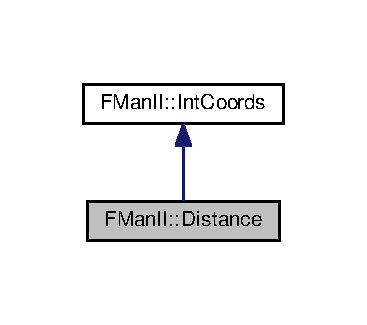
\includegraphics[width=176pt]{classFManII_1_1Distance__inherit__graph}
\end{center}
\end{figure}


Collaboration diagram for F\+Man\+II\+:\+:Distance\+:\nopagebreak
\begin{figure}[H]
\begin{center}
\leavevmode
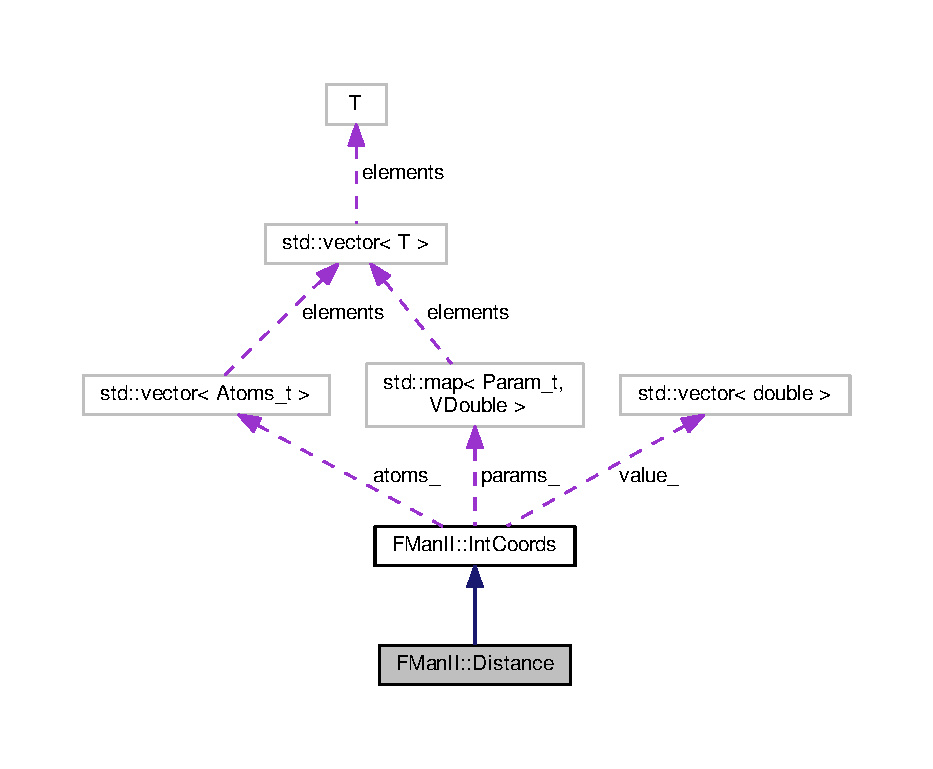
\includegraphics[width=350pt]{classFManII_1_1Distance__coll__graph}
\end{center}
\end{figure}
\subsection*{Public Member Functions}
\begin{DoxyCompactItemize}
\item 
{\bfseries Distance} (std\+::shared\+\_\+ptr$<$ const \hyperlink{classFManII_1_1IntCoords_af42df2795dec16350f908cfd5ac2ef06}{V\+Double} $>$ Carts)\hypertarget{classFManII_1_1Distance_a4266618c8a07a07ac8c29e22f2c289b7}{}\label{classFManII_1_1Distance_a4266618c8a07a07ac8c29e22f2c289b7}

\item 
{\footnotesize template$<$typename... args$>$ }\\void \hyperlink{classFManII_1_1IntCoords_aaa13717daa2c47a00c56e8dcb18896b6}{add\+\_\+coord} (const \hyperlink{classFManII_1_1IntCoords_a59ab25571f774fca97644a2ce5ade359}{Atoms\+\_\+t} \&coord, \hyperlink{namespaceFManII_ab331802fde4c5f2564443f1704c25363}{Param\+\_\+t} param, double pvalue, args...\+other\+\_\+params)
\begin{DoxyCompactList}\small\item\em The call to add a coordinate to this Int\+Coord. \end{DoxyCompactList}\item 
const \hyperlink{classFManII_1_1IntCoords_af42df2795dec16350f908cfd5ac2ef06}{V\+Double} \& \hyperlink{classFManII_1_1IntCoords_a8b36508bebeb262d2c41bed1301ad9f9}{values} () const \hypertarget{classFManII_1_1IntCoords_a8b36508bebeb262d2c41bed1301ad9f9}{}\label{classFManII_1_1IntCoords_a8b36508bebeb262d2c41bed1301ad9f9}

\begin{DoxyCompactList}\small\item\em Returns the array of coordinates. \end{DoxyCompactList}\item 
const \hyperlink{classFManII_1_1IntCoords_af42df2795dec16350f908cfd5ac2ef06}{V\+Double} \& \hyperlink{classFManII_1_1IntCoords_ac107ad541179d838052f37538883671a}{params} (\hyperlink{namespaceFManII_ab331802fde4c5f2564443f1704c25363}{Param\+\_\+t} pt) const \hypertarget{classFManII_1_1IntCoords_ac107ad541179d838052f37538883671a}{}\label{classFManII_1_1IntCoords_ac107ad541179d838052f37538883671a}

\begin{DoxyCompactList}\small\item\em Returns the array of a particular parameter. \end{DoxyCompactList}\end{DoxyCompactItemize}
\subsection*{Protected Types}
\begin{DoxyCompactItemize}
\item 
using \hyperlink{classFManII_1_1IntCoords_a59ab25571f774fca97644a2ce5ade359}{Atoms\+\_\+t} = std\+::vector$<$ size\+\_\+t $>$\hypertarget{classFManII_1_1IntCoords_a59ab25571f774fca97644a2ce5ade359}{}\label{classFManII_1_1IntCoords_a59ab25571f774fca97644a2ce5ade359}

\begin{DoxyCompactList}\small\item\em Typedef for the set of atoms in an Int\+Coord. \end{DoxyCompactList}\item 
using \hyperlink{classFManII_1_1IntCoords_af42df2795dec16350f908cfd5ac2ef06}{V\+Double} = std\+::vector$<$ double $>$\hypertarget{classFManII_1_1IntCoords_af42df2795dec16350f908cfd5ac2ef06}{}\label{classFManII_1_1IntCoords_af42df2795dec16350f908cfd5ac2ef06}

\begin{DoxyCompactList}\small\item\em Typedef for a vector of doubles. \end{DoxyCompactList}\end{DoxyCompactItemize}
\subsection*{Protected Member Functions}
\begin{DoxyCompactItemize}
\item 
\hyperlink{classFManII_1_1IntCoords_af42df2795dec16350f908cfd5ac2ef06}{V\+Double} \hyperlink{classFManII_1_1Distance_a16c3e07ee527b33379311e9099ec6497}{compute\+\_\+value} (size\+\_\+t deriv\+\_\+i, \hyperlink{classFManII_1_1IntCoords_a59ab25571f774fca97644a2ce5ade359}{Atoms\+\_\+t} coord\+\_\+i) const 
\begin{DoxyCompactList}\small\item\em Overridden by the derived class so that it computes the i-\/th derivative of the coordinate which involves the specified atoms. \end{DoxyCompactList}\item 
void \hyperlink{classFManII_1_1IntCoords_a21ae6c2eb4a0dbea71a402f399061d5b}{add\+\_\+coord} (const \hyperlink{classFManII_1_1IntCoords_a59ab25571f774fca97644a2ce5ade359}{Atoms\+\_\+t} \&coord)\hypertarget{classFManII_1_1IntCoords_a21ae6c2eb4a0dbea71a402f399061d5b}{}\label{classFManII_1_1IntCoords_a21ae6c2eb4a0dbea71a402f399061d5b}

\begin{DoxyCompactList}\small\item\em Recursion end point. \end{DoxyCompactList}\end{DoxyCompactItemize}
\subsection*{Protected Attributes}
\begin{DoxyCompactItemize}
\item 
size\+\_\+t \hyperlink{classFManII_1_1IntCoords_a3fb097438609927dda0f1a049ff61a72}{natoms\+\_\+}\hypertarget{classFManII_1_1IntCoords_a3fb097438609927dda0f1a049ff61a72}{}\label{classFManII_1_1IntCoords_a3fb097438609927dda0f1a049ff61a72}

\begin{DoxyCompactList}\small\item\em The number of atoms this coordinate depends on. \end{DoxyCompactList}\item 
std\+::shared\+\_\+ptr$<$ const \hyperlink{classFManII_1_1IntCoords_af42df2795dec16350f908cfd5ac2ef06}{V\+Double} $>$ \hyperlink{classFManII_1_1IntCoords_a54cd82d40213e7c85ea338b79438b22a}{carts\+\_\+}\hypertarget{classFManII_1_1IntCoords_a54cd82d40213e7c85ea338b79438b22a}{}\label{classFManII_1_1IntCoords_a54cd82d40213e7c85ea338b79438b22a}

\begin{DoxyCompactList}\small\item\em The cartesian coordinates of the system in a.\+u. \end{DoxyCompactList}\item 
\hyperlink{classFManII_1_1IntCoords_af42df2795dec16350f908cfd5ac2ef06}{V\+Double} \hyperlink{classFManII_1_1IntCoords_a1dfc726f1b6060c0f4e26eafb51953f9}{value\+\_\+}\hypertarget{classFManII_1_1IntCoords_a1dfc726f1b6060c0f4e26eafb51953f9}{}\label{classFManII_1_1IntCoords_a1dfc726f1b6060c0f4e26eafb51953f9}

\begin{DoxyCompactList}\small\item\em The actual length of the bond, or angle of the angle, etc. \end{DoxyCompactList}\item 
std\+::vector$<$ \hyperlink{classFManII_1_1IntCoords_a59ab25571f774fca97644a2ce5ade359}{Atoms\+\_\+t} $>$ \hyperlink{classFManII_1_1IntCoords_a4f7c142879fb222c66ae6968160d36c0}{atoms\+\_\+}\hypertarget{classFManII_1_1IntCoords_a4f7c142879fb222c66ae6968160d36c0}{}\label{classFManII_1_1IntCoords_a4f7c142879fb222c66ae6968160d36c0}

\begin{DoxyCompactList}\small\item\em The atom numbers associated with each value. \end{DoxyCompactList}\item 
std\+::map$<$ \hyperlink{namespaceFManII_ab331802fde4c5f2564443f1704c25363}{Param\+\_\+t}, \hyperlink{classFManII_1_1IntCoords_af42df2795dec16350f908cfd5ac2ef06}{V\+Double} $>$ \hyperlink{classFManII_1_1IntCoords_ab1a5fd9c10badbeb02ac40516a7183cc}{params\+\_\+}\hypertarget{classFManII_1_1IntCoords_ab1a5fd9c10badbeb02ac40516a7183cc}{}\label{classFManII_1_1IntCoords_ab1a5fd9c10badbeb02ac40516a7183cc}

\begin{DoxyCompactList}\small\item\em The parameters associated with this set of internal coordinates. \end{DoxyCompactList}\end{DoxyCompactItemize}


\subsection{Detailed Description}
Implements derivatives for distance between points. See \hyperlink{distance}{Distance Class} for more detail. 

\subsection{Member Function Documentation}
\index{F\+Man\+I\+I\+::\+Distance@{F\+Man\+I\+I\+::\+Distance}!add\+\_\+coord@{add\+\_\+coord}}
\index{add\+\_\+coord@{add\+\_\+coord}!F\+Man\+I\+I\+::\+Distance@{F\+Man\+I\+I\+::\+Distance}}
\subsubsection[{\texorpdfstring{add\+\_\+coord(const Atoms\+\_\+t \&coord, Param\+\_\+t param, double pvalue, args...\+other\+\_\+params)}{add_coord(const Atoms_t &coord, Param_t param, double pvalue, args...other_params)}}]{\setlength{\rightskip}{0pt plus 5cm}template$<$typename... args$>$ void F\+Man\+I\+I\+::\+Int\+Coords\+::add\+\_\+coord (
\begin{DoxyParamCaption}
\item[{const {\bf Atoms\+\_\+t} \&}]{coord, }
\item[{{\bf Param\+\_\+t}}]{param, }
\item[{double}]{pvalue, }
\item[{args...}]{other\+\_\+params}
\end{DoxyParamCaption}
)\hspace{0.3cm}{\ttfamily [inline]}, {\ttfamily [inherited]}}\hypertarget{classFManII_1_1IntCoords_aaa13717daa2c47a00c56e8dcb18896b6}{}\label{classFManII_1_1IntCoords_aaa13717daa2c47a00c56e8dcb18896b6}
Don\textquotesingle{}t be offput by the signature using this function is pretty easy. The first argument is the atoms in this coordinate. The remaining 2N arguments are the N parameters associated with this coordinate. They must be in the order parameter type, value of that parameter, next parameter type, value of the next parameter, etc. You will get a compile time error if you do not supply pairs for each parameter or if you mix up the order.

Point is usage looks like this\+: 
\begin{DoxyCode}
\textcolor{comment}{//Assume these are already made instances of IntCoords}
\hyperlink{classFManII_1_1IntCoords_aff5b80e7f579dd8aeac5200942b4db87}{IntCoords} MyBonds,MyAngles;

\textcolor{comment}{//Adds a bond between atoms 1 and 2 with a force constant of 3.4}
MyBonds.add\_coord(\{1,2\},\hyperlink{namespaceFManII_ab331802fde4c5f2564443f1704c25363acce4c4e3a7008d8a210e0950f0ae6646}{Param\_t::K},3.4);

\textcolor{comment}{//Adds an angle among atoms 1, 2, and 3 with force constant 3.3}
MyAngles.add\_coord(\{1,2,3\},\hyperlink{namespaceFManII_ab331802fde4c5f2564443f1704c25363acce4c4e3a7008d8a210e0950f0ae6646}{Param\_t::K},3.3);
\end{DoxyCode}



\begin{DoxyParams}[1]{Parameters}
\mbox{\tt in}  & {\em coord} & An array of the atoms in the coordinate. Numbers must correspond to the order given at instance creation \\
\hline
\mbox{\tt in}  & {\em param} & The type of the parameter, e.\+g. force constant \\
\hline
\mbox{\tt in}  & {\em pvalue} & The value of the parameter in a.\+u. \\
\hline
\mbox{\tt in}  & {\em other\+\_\+params} & Remaining parameter type, parameter value pairs \\
\hline
\end{DoxyParams}
\index{F\+Man\+I\+I\+::\+Distance@{F\+Man\+I\+I\+::\+Distance}!compute\+\_\+value@{compute\+\_\+value}}
\index{compute\+\_\+value@{compute\+\_\+value}!F\+Man\+I\+I\+::\+Distance@{F\+Man\+I\+I\+::\+Distance}}
\subsubsection[{\texorpdfstring{compute\+\_\+value(size\+\_\+t deriv\+\_\+i, Atoms\+\_\+t coord\+\_\+i) const }{compute_value(size_t deriv_i, Atoms_t coord_i) const }}]{\setlength{\rightskip}{0pt plus 5cm}{\bf Distance\+::\+V\+Double} F\+Man\+I\+I\+::\+Distance\+::compute\+\_\+value (
\begin{DoxyParamCaption}
\item[{size\+\_\+t}]{deriv\+\_\+i, }
\item[{{\bf Atoms\+\_\+t}}]{coord\+\_\+i}
\end{DoxyParamCaption}
) const\hspace{0.3cm}{\ttfamily [protected]}, {\ttfamily [virtual]}}\hypertarget{classFManII_1_1Distance_a16c3e07ee527b33379311e9099ec6497}{}\label{classFManII_1_1Distance_a16c3e07ee527b33379311e9099ec6497}
We provide you the derivative order and the coordinate number. At the moment I am assuming that while computing the value some of the parameters can be baked into the value to simplify things later. Specifically I am assuming that the 0-\/th order derivative can just return the difference between the actual value and the equilibrium distance for bonds, angles, and Urey-\/\+Bradley terms.


\begin{DoxyParams}[1]{Parameters}
\mbox{\tt in}  & {\em deriv\+\_\+i} & What order-\/th derivative should you return? \\
\hline
\mbox{\tt in}  & {\em coord\+\_\+i} & Which coordinate are you taking the derivative of? \\
\hline
\end{DoxyParams}
\begin{DoxyReturn}{Returns}
A $(3N)^{i}$ long array of the derivatives in the order\+: x of the first atom in the coord, y of the first atom in the coord, z of the first atom in the coord, x of the second atom in the coord,... along each of the $i$ dimensions of the derivative. 
\end{DoxyReturn}


Implements \hyperlink{classFManII_1_1IntCoords_ae8d77a3410edbc99357a2289feeec510}{F\+Man\+I\+I\+::\+Int\+Coords}.



The documentation for this class was generated from the following files\+:\begin{DoxyCompactItemize}
\item 
\hyperlink{Distance_8hpp}{Distance.\+hpp}\item 
Distance.\+cpp\end{DoxyCompactItemize}

\hypertarget{classFManII_1_1FFTerm}{}\section{F\+Man\+II\+:\+:F\+F\+Term$<$ Model\+\_\+t, Coord\+\_\+t $>$ Class Template Reference}
\label{classFManII_1_1FFTerm}\index{F\+Man\+I\+I\+::\+F\+F\+Term$<$ Model\+\_\+t, Coord\+\_\+t $>$@{F\+Man\+I\+I\+::\+F\+F\+Term$<$ Model\+\_\+t, Coord\+\_\+t $>$}}


{\ttfamily \#include $<$F\+F\+Term.\+hpp$>$}



\subsection{Detailed Description}
\subsubsection*{template$<$typename Model\+\_\+t, typename Coord\+\_\+t$>$\\*
class F\+Man\+I\+I\+::\+F\+F\+Term$<$ Model\+\_\+t, Coord\+\_\+t $>$}

The class responsible for computing derivatives of a force field term

All energetic terms in a forcefield depend on some generic coordinate $q$, which itself depends on the standard Cartesian coordinates of the system. Consequentially, the first derivative of the energy with respect to one of these coordinates, say $x$ is\+: \[ \frac{\partial E(q)}{\partial x}=\frac{\partial f(q)}{\partial q} \frac{\partial q}{\partial x}, \] where $f(q)$ is the functional form of the term (harmonic oscillator, Fourier series, etc). The second derivative with respect to $x$ and $y$ is then\+: \[ \frac{\partial^2 E(q)}{\partial x\partial y}= \frac{\partial^2 f(q)}{\partial q^2}\frac{\partial q}{\partial x} \frac{\partial q}{\partial y}+ \frac{\partial f(q)}{\partial q} \frac{\partial q^2}{\partial x\partial y} \]

This class is responsible for handeling these derivative manipulations in a generic way. Eventually I probably will want to expand this to include higher-\/order terms like those in the M\+M4 series which involve cross-\/terms between parameters. In those cases the chain rule seen here needs generalized to multiple $q$ and I anticipate there being an additional template type parameter.


\begin{DoxyParams}[1]{Parameters}
\mbox{\tt in}  & {\em Model\+\_\+t} & The class type of our functional form \\
\hline
\mbox{\tt in}  & {\em Coord\+\_\+t} & The class type of the coordinate this term depends on \\
\hline
\end{DoxyParams}


The documentation for this class was generated from the following file\+:\begin{DoxyCompactItemize}
\item 
\hyperlink{FFTerm_8hpp}{F\+F\+Term.\+hpp}\end{DoxyCompactItemize}

\hypertarget{structFManII_1_1FourierSeries}{}\section{F\+Man\+II\+:\+:Fourier\+Series Struct Reference}
\label{structFManII_1_1FourierSeries}\index{F\+Man\+I\+I\+::\+Fourier\+Series@{F\+Man\+I\+I\+::\+Fourier\+Series}}


Implements a Fourier Series model potential.  




{\ttfamily \#include $<$Fourier\+Series.\+hpp$>$}

\subsection*{Public Member Functions}
\begin{DoxyCompactItemize}
\item 
std\+::vector$<$ double $>$ \hyperlink{structFManII_1_1FourierSeries_aabd5e4a496079dcbba386dec65a88cdd}{deriv} (const std\+::vector$<$ double $>$ \&Qs, const std\+::vector$<$ double $>$ \&Vs, const std\+::vector$<$ double $>$ \&ns, unsigned int Order=0) const 
\end{DoxyCompactItemize}


\subsection{Detailed Description}
See \hyperlink{fourier}{Fourier Series} for details regarding conventions etc. 

\subsection{Member Function Documentation}
\index{F\+Man\+I\+I\+::\+Fourier\+Series@{F\+Man\+I\+I\+::\+Fourier\+Series}!deriv@{deriv}}
\index{deriv@{deriv}!F\+Man\+I\+I\+::\+Fourier\+Series@{F\+Man\+I\+I\+::\+Fourier\+Series}}
\subsubsection[{\texorpdfstring{deriv(const std\+::vector$<$ double $>$ \&\+Qs, const std\+::vector$<$ double $>$ \&\+Vs, const std\+::vector$<$ double $>$ \&ns, unsigned int Order=0) const }{deriv(const std::vector< double > &Qs, const std::vector< double > &Vs, const std::vector< double > &ns, unsigned int Order=0) const }}]{\setlength{\rightskip}{0pt plus 5cm}Return\+\_\+t F\+Man\+I\+I\+::\+Fourier\+Series\+::deriv (
\begin{DoxyParamCaption}
\item[{const std\+::vector$<$ double $>$ \&}]{Qs, }
\item[{const std\+::vector$<$ double $>$ \&}]{Vs, }
\item[{const std\+::vector$<$ double $>$ \&}]{ns, }
\item[{unsigned int}]{Order = {\ttfamily 0}}
\end{DoxyParamCaption}
) const}\hypertarget{structFManII_1_1FourierSeries_aabd5e4a496079dcbba386dec65a88cdd}{}\label{structFManII_1_1FourierSeries_aabd5e4a496079dcbba386dec65a88cdd}
Computes the derivative of the energy of a \hyperlink{structFManII_1_1FourierSeries}{Fourier\+Series}

\begin{DoxyNote}{Note}
This function expects all quantities to be in atomic units
\end{DoxyNote}

\begin{DoxyParams}[1]{Parameters}
\mbox{\tt in}  & {\em Qs} & An N element vector such that the i-\/th element is the value of the i-\/th coordinate (torsion, impropertorsion, etc.) with the periodicity and phase shift already evalutate, i.\+e. give me n$\ast$phi-\/gamma for each angle \\
\hline
\mbox{\tt in}  & {\em Vs} & An N element vector such that the i-\/th element is the value of the i-\/th coordinate\textquotesingle{}s amplitude \\
\hline
\mbox{\tt in}  & {\em ns} & A N element vector such that the i-\/th element is the value of the i-\/th coordinate\textquotesingle{}s periodicity \\
\hline
\mbox{\tt in}  & {\em Order} & What order derivative are we returning? \\
\hline
\end{DoxyParams}
\begin{DoxyReturn}{Returns}
The derivative in atomic units. 
\end{DoxyReturn}


The documentation for this struct was generated from the following files\+:\begin{DoxyCompactItemize}
\item 
\hyperlink{FourierSeries_8hpp}{Fourier\+Series.\+hpp}\item 
Fourier\+Series.\+cpp\end{DoxyCompactItemize}

\hypertarget{structFManII_1_1HarmonicOscillator}{}\section{F\+Man\+II\+:\+:Harmonic\+Oscillator Struct Reference}
\label{structFManII_1_1HarmonicOscillator}\index{F\+Man\+I\+I\+::\+Harmonic\+Oscillator@{F\+Man\+I\+I\+::\+Harmonic\+Oscillator}}


Implements the harmonic oscillator model potential.  




{\ttfamily \#include $<$Harmonic\+Oscillator.\+hpp$>$}

\subsection*{Public Member Functions}
\begin{DoxyCompactItemize}
\item 
std\+::vector$<$ double $>$ \hyperlink{structFManII_1_1HarmonicOscillator_a3d363faf1dee2c2d5d26993f8235fc57}{deriv} (const std\+::vector$<$ double $>$ \&Qs, const std\+::vector$<$ double $>$ \&Ks, unsigned int Order=0) const 
\end{DoxyCompactItemize}


\subsection{Detailed Description}
See \hyperlink{HO}{Harmonic Oscillator} for details regarding conventions etc. 

\subsection{Member Function Documentation}
\index{F\+Man\+I\+I\+::\+Harmonic\+Oscillator@{F\+Man\+I\+I\+::\+Harmonic\+Oscillator}!deriv@{deriv}}
\index{deriv@{deriv}!F\+Man\+I\+I\+::\+Harmonic\+Oscillator@{F\+Man\+I\+I\+::\+Harmonic\+Oscillator}}
\subsubsection[{\texorpdfstring{deriv(const std\+::vector$<$ double $>$ \&\+Qs, const std\+::vector$<$ double $>$ \&\+Ks, unsigned int Order=0) const }{deriv(const std::vector< double > &Qs, const std::vector< double > &Ks, unsigned int Order=0) const }}]{\setlength{\rightskip}{0pt plus 5cm}Return\+\_\+t F\+Man\+I\+I\+::\+Harmonic\+Oscillator\+::deriv (
\begin{DoxyParamCaption}
\item[{const std\+::vector$<$ double $>$ \&}]{Qs, }
\item[{const std\+::vector$<$ double $>$ \&}]{Ks, }
\item[{unsigned int}]{Order = {\ttfamily 0}}
\end{DoxyParamCaption}
) const}\hypertarget{structFManII_1_1HarmonicOscillator_a3d363faf1dee2c2d5d26993f8235fc57}{}\label{structFManII_1_1HarmonicOscillator_a3d363faf1dee2c2d5d26993f8235fc57}
Computes the derivative of the energy of a Harmonic Oscillator

\begin{DoxyNote}{Note}
This function expects all quantities to be in atomic units
\end{DoxyNote}

\begin{DoxyParams}[1]{Parameters}
\mbox{\tt in}  & {\em Qs} & An N element vector such that the i-\/th element is the value of the i-\/th coordinate (bond-\/length, angle, etc.) \\
\hline
\mbox{\tt in}  & {\em Ks} & An N element vector such that the i-\/th element is the value of the i-\/th coordinate\textquotesingle{}s force constant \\
\hline
\mbox{\tt in}  & {\em Order} & What order derivative are we returning? \\
\hline
\end{DoxyParams}
\begin{DoxyReturn}{Returns}
The derivative in atomic units. 
\end{DoxyReturn}


The documentation for this struct was generated from the following files\+:\begin{DoxyCompactItemize}
\item 
\hyperlink{HarmonicOscillator_8hpp}{Harmonic\+Oscillator.\+hpp}\item 
Harmonic\+Oscillator.\+cpp\end{DoxyCompactItemize}

\hypertarget{classFManII_1_1IntCoords}{}\section{F\+Man\+II\+:\+:Int\+Coords Class Reference}
\label{classFManII_1_1IntCoords}\index{F\+Man\+I\+I\+::\+Int\+Coords@{F\+Man\+I\+I\+::\+Int\+Coords}}


A base class designed to provide basic functionality to things like bonds, angles, etc.  




{\ttfamily \#include $<$Internal\+Coordinates.\+hpp$>$}



Inheritance diagram for F\+Man\+II\+:\+:Int\+Coords\+:\nopagebreak
\begin{figure}[H]
\begin{center}
\leavevmode
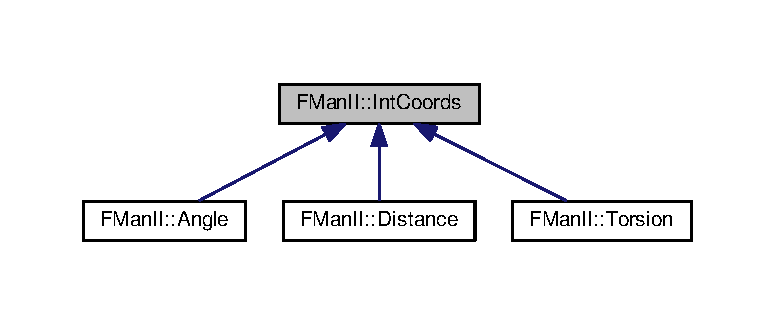
\includegraphics[width=350pt]{classFManII_1_1IntCoords__inherit__graph}
\end{center}
\end{figure}


Collaboration diagram for F\+Man\+II\+:\+:Int\+Coords\+:\nopagebreak
\begin{figure}[H]
\begin{center}
\leavevmode
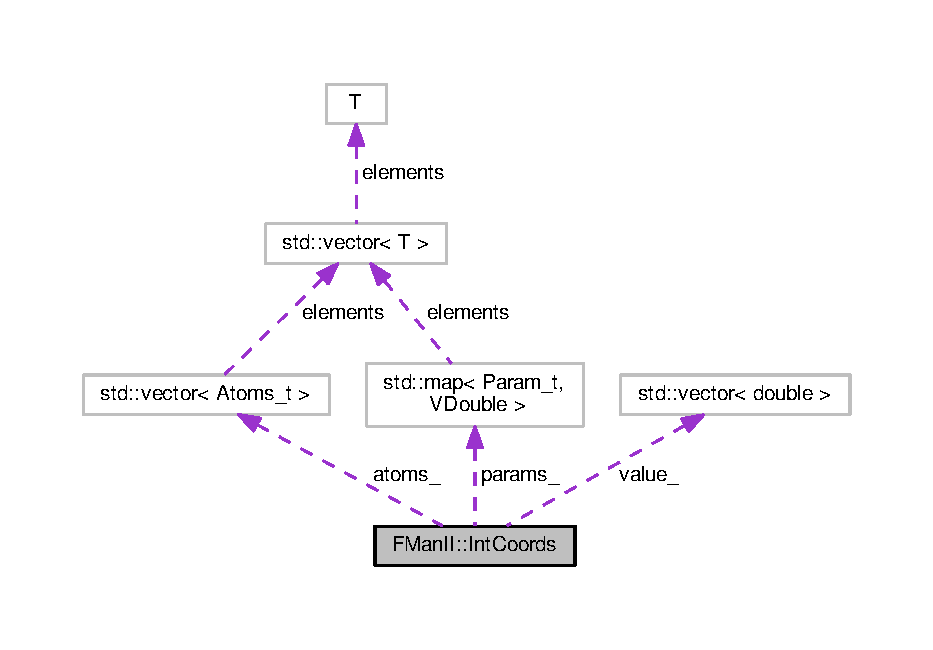
\includegraphics[width=350pt]{classFManII_1_1IntCoords__coll__graph}
\end{center}
\end{figure}
\subsection*{Public Member Functions}
\begin{DoxyCompactItemize}
\item 
{\footnotesize template$<$typename... args$>$ }\\void \hyperlink{classFManII_1_1IntCoords_aaa13717daa2c47a00c56e8dcb18896b6}{add\+\_\+coord} (const \hyperlink{classFManII_1_1IntCoords_a59ab25571f774fca97644a2ce5ade359}{Atoms\+\_\+t} \&coord, \hyperlink{namespaceFManII_ab331802fde4c5f2564443f1704c25363}{Param\+\_\+t} param, double pvalue, args...\+other\+\_\+params)
\begin{DoxyCompactList}\small\item\em The call to add a coordinate to this Int\+Coord. \end{DoxyCompactList}\item 
const \hyperlink{classFManII_1_1IntCoords_af42df2795dec16350f908cfd5ac2ef06}{V\+Double} \& \hyperlink{classFManII_1_1IntCoords_a8b36508bebeb262d2c41bed1301ad9f9}{values} () const \hypertarget{classFManII_1_1IntCoords_a8b36508bebeb262d2c41bed1301ad9f9}{}\label{classFManII_1_1IntCoords_a8b36508bebeb262d2c41bed1301ad9f9}

\begin{DoxyCompactList}\small\item\em Returns the array of coordinates. \end{DoxyCompactList}\item 
const \hyperlink{classFManII_1_1IntCoords_af42df2795dec16350f908cfd5ac2ef06}{V\+Double} \& \hyperlink{classFManII_1_1IntCoords_ac107ad541179d838052f37538883671a}{params} (\hyperlink{namespaceFManII_ab331802fde4c5f2564443f1704c25363}{Param\+\_\+t} pt) const \hypertarget{classFManII_1_1IntCoords_ac107ad541179d838052f37538883671a}{}\label{classFManII_1_1IntCoords_ac107ad541179d838052f37538883671a}

\begin{DoxyCompactList}\small\item\em Returns the array of a particular parameter. \end{DoxyCompactList}\item 
virtual \hyperlink{classFManII_1_1IntCoords_ad31ec2a0d63bb2fc33677057546d2763}{$\sim$\+Int\+Coords} ()\hypertarget{classFManII_1_1IntCoords_ad31ec2a0d63bb2fc33677057546d2763}{}\label{classFManII_1_1IntCoords_ad31ec2a0d63bb2fc33677057546d2763}

\begin{DoxyCompactList}\small\item\em Virtual Dtor so compiler doesn\textquotesingle{}t complain, but does nothing. \end{DoxyCompactList}\end{DoxyCompactItemize}
\subsection*{Protected Types}
\begin{DoxyCompactItemize}
\item 
using \hyperlink{classFManII_1_1IntCoords_a59ab25571f774fca97644a2ce5ade359}{Atoms\+\_\+t} = std\+::vector$<$ size\+\_\+t $>$\hypertarget{classFManII_1_1IntCoords_a59ab25571f774fca97644a2ce5ade359}{}\label{classFManII_1_1IntCoords_a59ab25571f774fca97644a2ce5ade359}

\begin{DoxyCompactList}\small\item\em Typedef for the set of atoms in an Int\+Coord. \end{DoxyCompactList}\item 
using \hyperlink{classFManII_1_1IntCoords_af42df2795dec16350f908cfd5ac2ef06}{V\+Double} = std\+::vector$<$ double $>$\hypertarget{classFManII_1_1IntCoords_af42df2795dec16350f908cfd5ac2ef06}{}\label{classFManII_1_1IntCoords_af42df2795dec16350f908cfd5ac2ef06}

\begin{DoxyCompactList}\small\item\em Typedef for a vector of doubles. \end{DoxyCompactList}\end{DoxyCompactItemize}
\subsection*{Protected Member Functions}
\begin{DoxyCompactItemize}
\item 
virtual \hyperlink{classFManII_1_1IntCoords_af42df2795dec16350f908cfd5ac2ef06}{V\+Double} \hyperlink{classFManII_1_1IntCoords_ae8d77a3410edbc99357a2289feeec510}{compute\+\_\+value} (size\+\_\+t deriv\+\_\+i, \hyperlink{classFManII_1_1IntCoords_a59ab25571f774fca97644a2ce5ade359}{Atoms\+\_\+t} coord\+\_\+i) const =0
\begin{DoxyCompactList}\small\item\em Overridden by the derived class so that it computes the i-\/th derivative of the coordinate which involves the specified atoms. \end{DoxyCompactList}\item 
void \hyperlink{classFManII_1_1IntCoords_a21ae6c2eb4a0dbea71a402f399061d5b}{add\+\_\+coord} (const \hyperlink{classFManII_1_1IntCoords_a59ab25571f774fca97644a2ce5ade359}{Atoms\+\_\+t} \&coord)\hypertarget{classFManII_1_1IntCoords_a21ae6c2eb4a0dbea71a402f399061d5b}{}\label{classFManII_1_1IntCoords_a21ae6c2eb4a0dbea71a402f399061d5b}

\begin{DoxyCompactList}\small\item\em Recursion end point. \end{DoxyCompactList}\item 
\hyperlink{classFManII_1_1IntCoords_aff5b80e7f579dd8aeac5200942b4db87}{Int\+Coords} (size\+\_\+t N\+Atoms, std\+::shared\+\_\+ptr$<$ const \hyperlink{classFManII_1_1IntCoords_af42df2795dec16350f908cfd5ac2ef06}{V\+Double} $>$ Carts)\hypertarget{classFManII_1_1IntCoords_aff5b80e7f579dd8aeac5200942b4db87}{}\label{classFManII_1_1IntCoords_aff5b80e7f579dd8aeac5200942b4db87}

\begin{DoxyCompactList}\small\item\em {\ttfamily Carts} is coordinates of the molecule in a.\+u. in a N\+Atoms X 3 array \end{DoxyCompactList}\end{DoxyCompactItemize}
\subsection*{Protected Attributes}
\begin{DoxyCompactItemize}
\item 
size\+\_\+t \hyperlink{classFManII_1_1IntCoords_a3fb097438609927dda0f1a049ff61a72}{natoms\+\_\+}\hypertarget{classFManII_1_1IntCoords_a3fb097438609927dda0f1a049ff61a72}{}\label{classFManII_1_1IntCoords_a3fb097438609927dda0f1a049ff61a72}

\begin{DoxyCompactList}\small\item\em The number of atoms this coordinate depends on. \end{DoxyCompactList}\item 
std\+::shared\+\_\+ptr$<$ const \hyperlink{classFManII_1_1IntCoords_af42df2795dec16350f908cfd5ac2ef06}{V\+Double} $>$ \hyperlink{classFManII_1_1IntCoords_a54cd82d40213e7c85ea338b79438b22a}{carts\+\_\+}\hypertarget{classFManII_1_1IntCoords_a54cd82d40213e7c85ea338b79438b22a}{}\label{classFManII_1_1IntCoords_a54cd82d40213e7c85ea338b79438b22a}

\begin{DoxyCompactList}\small\item\em The cartesian coordinates of the system in a.\+u. \end{DoxyCompactList}\item 
\hyperlink{classFManII_1_1IntCoords_af42df2795dec16350f908cfd5ac2ef06}{V\+Double} \hyperlink{classFManII_1_1IntCoords_a1dfc726f1b6060c0f4e26eafb51953f9}{value\+\_\+}\hypertarget{classFManII_1_1IntCoords_a1dfc726f1b6060c0f4e26eafb51953f9}{}\label{classFManII_1_1IntCoords_a1dfc726f1b6060c0f4e26eafb51953f9}

\begin{DoxyCompactList}\small\item\em The actual length of the bond, or angle of the angle, etc. \end{DoxyCompactList}\item 
std\+::vector$<$ \hyperlink{classFManII_1_1IntCoords_a59ab25571f774fca97644a2ce5ade359}{Atoms\+\_\+t} $>$ \hyperlink{classFManII_1_1IntCoords_a4f7c142879fb222c66ae6968160d36c0}{atoms\+\_\+}\hypertarget{classFManII_1_1IntCoords_a4f7c142879fb222c66ae6968160d36c0}{}\label{classFManII_1_1IntCoords_a4f7c142879fb222c66ae6968160d36c0}

\begin{DoxyCompactList}\small\item\em The atom numbers associated with each value. \end{DoxyCompactList}\item 
std\+::map$<$ \hyperlink{namespaceFManII_ab331802fde4c5f2564443f1704c25363}{Param\+\_\+t}, \hyperlink{classFManII_1_1IntCoords_af42df2795dec16350f908cfd5ac2ef06}{V\+Double} $>$ \hyperlink{classFManII_1_1IntCoords_ab1a5fd9c10badbeb02ac40516a7183cc}{params\+\_\+}\hypertarget{classFManII_1_1IntCoords_ab1a5fd9c10badbeb02ac40516a7183cc}{}\label{classFManII_1_1IntCoords_ab1a5fd9c10badbeb02ac40516a7183cc}

\begin{DoxyCompactList}\small\item\em The parameters associated with this set of internal coordinates. \end{DoxyCompactList}\end{DoxyCompactItemize}


\subsection{Detailed Description}
Energetic terms in a force field rely on determining how far an internal coordinate, or Int\+Coord for short, is from an equilibrium value. These \hyperlink{classFManII_1_1IntCoords}{Int\+Coords} are things like bonds, angles, torsions, etc. and the force field maps the energetic cost of displacing these \hyperlink{classFManII_1_1IntCoords}{Int\+Coords} to simple functional forms. Hence it is key that we have a class to describe these internal coordinates.

Each instance of this class is designed to work with a single system. If you need to have \hyperlink{classFManII_1_1IntCoords}{Int\+Coords} for multiple systems make multiple instances. Basic workflow with this class is give it a natoms by 3 array of Cartesian coordinates at creation. At creation the order of the atoms is irrelevant, but after creation all further input with this class will refer to that ordering. Next an algorithm above this class locates the internal coordinate of choice (i.\+e. using the connectivity you find say a bond) you then add that bond to this class like\+: 
\begin{DoxyCode}
\hyperlink{classFManII_1_1IntCoords_aff5b80e7f579dd8aeac5200942b4db87}{IntCoords} Bonds(System);
Bonds.add\_coord(\{1,2\},\hyperlink{namespaceFManII_ab331802fde4c5f2564443f1704c25363acce4c4e3a7008d8a210e0950f0ae6646}{Param\_t::K},value\_of\_K);
\end{DoxyCode}
 and similarly for other coordinates. 

\subsection{Member Function Documentation}
\index{F\+Man\+I\+I\+::\+Int\+Coords@{F\+Man\+I\+I\+::\+Int\+Coords}!add\+\_\+coord@{add\+\_\+coord}}
\index{add\+\_\+coord@{add\+\_\+coord}!F\+Man\+I\+I\+::\+Int\+Coords@{F\+Man\+I\+I\+::\+Int\+Coords}}
\subsubsection[{\texorpdfstring{add\+\_\+coord(const Atoms\+\_\+t \&coord, Param\+\_\+t param, double pvalue, args...\+other\+\_\+params)}{add_coord(const Atoms_t &coord, Param_t param, double pvalue, args...other_params)}}]{\setlength{\rightskip}{0pt plus 5cm}template$<$typename... args$>$ void F\+Man\+I\+I\+::\+Int\+Coords\+::add\+\_\+coord (
\begin{DoxyParamCaption}
\item[{const {\bf Atoms\+\_\+t} \&}]{coord, }
\item[{{\bf Param\+\_\+t}}]{param, }
\item[{double}]{pvalue, }
\item[{args...}]{other\+\_\+params}
\end{DoxyParamCaption}
)\hspace{0.3cm}{\ttfamily [inline]}}\hypertarget{classFManII_1_1IntCoords_aaa13717daa2c47a00c56e8dcb18896b6}{}\label{classFManII_1_1IntCoords_aaa13717daa2c47a00c56e8dcb18896b6}
Don\textquotesingle{}t be offput by the signature using this function is pretty easy. The first argument is the atoms in this coordinate. The remaining 2N arguments are the N parameters associated with this coordinate. They must be in the order parameter type, value of that parameter, next parameter type, value of the next parameter, etc. You will get a compile time error if you do not supply pairs for each parameter or if you mix up the order.

Point is usage looks like this\+: 
\begin{DoxyCode}
\textcolor{comment}{//Assume these are already made instances of IntCoords}
\hyperlink{classFManII_1_1IntCoords_aff5b80e7f579dd8aeac5200942b4db87}{IntCoords} MyBonds,MyAngles;

\textcolor{comment}{//Adds a bond between atoms 1 and 2 with a force constant of 3.4}
MyBonds.add\_coord(\{1,2\},\hyperlink{namespaceFManII_ab331802fde4c5f2564443f1704c25363acce4c4e3a7008d8a210e0950f0ae6646}{Param\_t::K},3.4);

\textcolor{comment}{//Adds an angle among atoms 1, 2, and 3 with force constant 3.3}
MyAngles.add\_coord(\{1,2,3\},\hyperlink{namespaceFManII_ab331802fde4c5f2564443f1704c25363acce4c4e3a7008d8a210e0950f0ae6646}{Param\_t::K},3.3);
\end{DoxyCode}



\begin{DoxyParams}[1]{Parameters}
\mbox{\tt in}  & {\em coord} & An array of the atoms in the coordinate. Numbers must correspond to the order given at instance creation \\
\hline
\mbox{\tt in}  & {\em param} & The type of the parameter, e.\+g. force constant \\
\hline
\mbox{\tt in}  & {\em pvalue} & The value of the parameter in a.\+u. \\
\hline
\mbox{\tt in}  & {\em other\+\_\+params} & Remaining parameter type, parameter value pairs \\
\hline
\end{DoxyParams}
\index{F\+Man\+I\+I\+::\+Int\+Coords@{F\+Man\+I\+I\+::\+Int\+Coords}!compute\+\_\+value@{compute\+\_\+value}}
\index{compute\+\_\+value@{compute\+\_\+value}!F\+Man\+I\+I\+::\+Int\+Coords@{F\+Man\+I\+I\+::\+Int\+Coords}}
\subsubsection[{\texorpdfstring{compute\+\_\+value(size\+\_\+t deriv\+\_\+i, Atoms\+\_\+t coord\+\_\+i) const =0}{compute_value(size_t deriv_i, Atoms_t coord_i) const =0}}]{\setlength{\rightskip}{0pt plus 5cm}virtual {\bf V\+Double} F\+Man\+I\+I\+::\+Int\+Coords\+::compute\+\_\+value (
\begin{DoxyParamCaption}
\item[{size\+\_\+t}]{deriv\+\_\+i, }
\item[{{\bf Atoms\+\_\+t}}]{coord\+\_\+i}
\end{DoxyParamCaption}
) const\hspace{0.3cm}{\ttfamily [protected]}, {\ttfamily [pure virtual]}}\hypertarget{classFManII_1_1IntCoords_ae8d77a3410edbc99357a2289feeec510}{}\label{classFManII_1_1IntCoords_ae8d77a3410edbc99357a2289feeec510}
We provide you the derivative order and the coordinate number. At the moment I am assuming that while computing the value some of the parameters can be baked into the value to simplify things later. Specifically I am assuming that the 0-\/th order derivative can just return the difference between the actual value and the equilibrium distance for bonds, angles, and Urey-\/\+Bradley terms.


\begin{DoxyParams}[1]{Parameters}
\mbox{\tt in}  & {\em deriv\+\_\+i} & What order-\/th derivative should you return? \\
\hline
\mbox{\tt in}  & {\em coord\+\_\+i} & Which coordinate are you taking the derivative of? \\
\hline
\end{DoxyParams}
\begin{DoxyReturn}{Returns}
A $(3N)^{i}$ long array of the derivatives in the order\+: x of the first atom in the coord, y of the first atom in the coord, z of the first atom in the coord, x of the second atom in the coord,... along each of the $i$ dimensions of the derivative. 
\end{DoxyReturn}


Implemented in \hyperlink{classFManII_1_1Angle_a48105b9c14048db6ccea1a410e8943f1}{F\+Man\+I\+I\+::\+Angle}, \hyperlink{classFManII_1_1Torsion_a5b1871f59ce0112bd17ee0add9bf993e}{F\+Man\+I\+I\+::\+Torsion}, and \hyperlink{classFManII_1_1Distance_a16c3e07ee527b33379311e9099ec6497}{F\+Man\+I\+I\+::\+Distance}.



The documentation for this class was generated from the following file\+:\begin{DoxyCompactItemize}
\item 
Internal\+Coordinates.\+hpp\end{DoxyCompactItemize}

\hypertarget{classFManII_1_1Torsion}{}\section{F\+Man\+II\+:\+:Torsion Class Reference}
\label{classFManII_1_1Torsion}\index{F\+Man\+I\+I\+::\+Torsion@{F\+Man\+I\+I\+::\+Torsion}}


{\ttfamily \#include $<$Torsion.\+hpp$>$}



Inheritance diagram for F\+Man\+II\+:\+:Torsion\+:\nopagebreak
\begin{figure}[H]
\begin{center}
\leavevmode
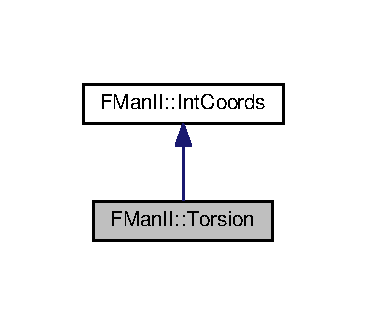
\includegraphics[width=176pt]{classFManII_1_1Torsion__inherit__graph}
\end{center}
\end{figure}


Collaboration diagram for F\+Man\+II\+:\+:Torsion\+:\nopagebreak
\begin{figure}[H]
\begin{center}
\leavevmode
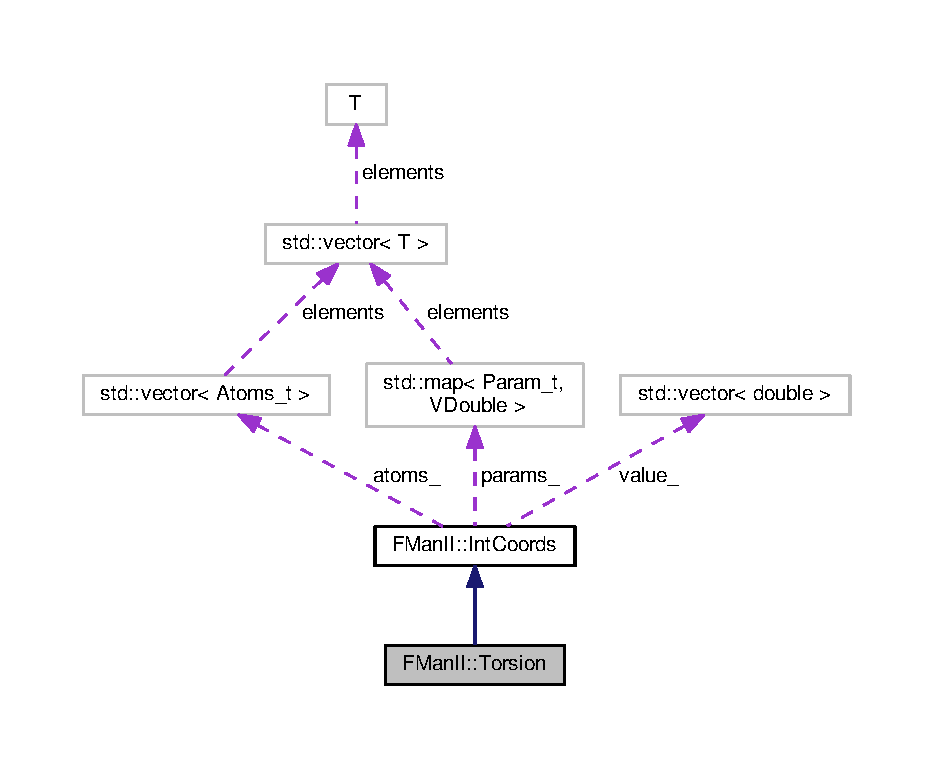
\includegraphics[width=350pt]{classFManII_1_1Torsion__coll__graph}
\end{center}
\end{figure}
\subsection*{Public Member Functions}
\begin{DoxyCompactItemize}
\item 
{\bfseries Torsion} (std\+::shared\+\_\+ptr$<$ const \hyperlink{classFManII_1_1IntCoords_af42df2795dec16350f908cfd5ac2ef06}{V\+Double} $>$ Carts)\hypertarget{classFManII_1_1Torsion_a28059ff2757f4ee3c353c7abed109db8}{}\label{classFManII_1_1Torsion_a28059ff2757f4ee3c353c7abed109db8}

\item 
{\footnotesize template$<$typename... args$>$ }\\void \hyperlink{classFManII_1_1IntCoords_aaa13717daa2c47a00c56e8dcb18896b6}{add\+\_\+coord} (const \hyperlink{classFManII_1_1IntCoords_a59ab25571f774fca97644a2ce5ade359}{Atoms\+\_\+t} \&coord, \hyperlink{namespaceFManII_ab331802fde4c5f2564443f1704c25363}{Param\+\_\+t} param, double pvalue, args...\+other\+\_\+params)
\begin{DoxyCompactList}\small\item\em The call to add a coordinate to this Int\+Coord. \end{DoxyCompactList}\item 
const \hyperlink{classFManII_1_1IntCoords_af42df2795dec16350f908cfd5ac2ef06}{V\+Double} \& \hyperlink{classFManII_1_1IntCoords_a8b36508bebeb262d2c41bed1301ad9f9}{values} () const \hypertarget{classFManII_1_1IntCoords_a8b36508bebeb262d2c41bed1301ad9f9}{}\label{classFManII_1_1IntCoords_a8b36508bebeb262d2c41bed1301ad9f9}

\begin{DoxyCompactList}\small\item\em Returns the array of coordinates. \end{DoxyCompactList}\item 
const \hyperlink{classFManII_1_1IntCoords_af42df2795dec16350f908cfd5ac2ef06}{V\+Double} \& \hyperlink{classFManII_1_1IntCoords_ac107ad541179d838052f37538883671a}{params} (\hyperlink{namespaceFManII_ab331802fde4c5f2564443f1704c25363}{Param\+\_\+t} pt) const \hypertarget{classFManII_1_1IntCoords_ac107ad541179d838052f37538883671a}{}\label{classFManII_1_1IntCoords_ac107ad541179d838052f37538883671a}

\begin{DoxyCompactList}\small\item\em Returns the array of a particular parameter. \end{DoxyCompactList}\end{DoxyCompactItemize}
\subsection*{Protected Types}
\begin{DoxyCompactItemize}
\item 
using \hyperlink{classFManII_1_1IntCoords_a59ab25571f774fca97644a2ce5ade359}{Atoms\+\_\+t} = std\+::vector$<$ size\+\_\+t $>$\hypertarget{classFManII_1_1IntCoords_a59ab25571f774fca97644a2ce5ade359}{}\label{classFManII_1_1IntCoords_a59ab25571f774fca97644a2ce5ade359}

\begin{DoxyCompactList}\small\item\em Typedef for the set of atoms in an Int\+Coord. \end{DoxyCompactList}\item 
using \hyperlink{classFManII_1_1IntCoords_af42df2795dec16350f908cfd5ac2ef06}{V\+Double} = std\+::vector$<$ double $>$\hypertarget{classFManII_1_1IntCoords_af42df2795dec16350f908cfd5ac2ef06}{}\label{classFManII_1_1IntCoords_af42df2795dec16350f908cfd5ac2ef06}

\begin{DoxyCompactList}\small\item\em Typedef for a vector of doubles. \end{DoxyCompactList}\end{DoxyCompactItemize}
\subsection*{Protected Member Functions}
\begin{DoxyCompactItemize}
\item 
\hyperlink{classFManII_1_1IntCoords_af42df2795dec16350f908cfd5ac2ef06}{V\+Double} \hyperlink{classFManII_1_1Torsion_a5b1871f59ce0112bd17ee0add9bf993e}{compute\+\_\+value} (size\+\_\+t deriv\+\_\+i, \hyperlink{classFManII_1_1IntCoords_a59ab25571f774fca97644a2ce5ade359}{Atoms\+\_\+t} coord\+\_\+i) const 
\begin{DoxyCompactList}\small\item\em Overridden by the derived class so that it computes the i-\/th derivative of the coordinate which involves the specified atoms. \end{DoxyCompactList}\item 
void \hyperlink{classFManII_1_1IntCoords_a21ae6c2eb4a0dbea71a402f399061d5b}{add\+\_\+coord} (const \hyperlink{classFManII_1_1IntCoords_a59ab25571f774fca97644a2ce5ade359}{Atoms\+\_\+t} \&coord)\hypertarget{classFManII_1_1IntCoords_a21ae6c2eb4a0dbea71a402f399061d5b}{}\label{classFManII_1_1IntCoords_a21ae6c2eb4a0dbea71a402f399061d5b}

\begin{DoxyCompactList}\small\item\em Recursion end point. \end{DoxyCompactList}\end{DoxyCompactItemize}
\subsection*{Protected Attributes}
\begin{DoxyCompactItemize}
\item 
size\+\_\+t \hyperlink{classFManII_1_1IntCoords_a3fb097438609927dda0f1a049ff61a72}{natoms\+\_\+}\hypertarget{classFManII_1_1IntCoords_a3fb097438609927dda0f1a049ff61a72}{}\label{classFManII_1_1IntCoords_a3fb097438609927dda0f1a049ff61a72}

\begin{DoxyCompactList}\small\item\em The number of atoms this coordinate depends on. \end{DoxyCompactList}\item 
std\+::shared\+\_\+ptr$<$ const \hyperlink{classFManII_1_1IntCoords_af42df2795dec16350f908cfd5ac2ef06}{V\+Double} $>$ \hyperlink{classFManII_1_1IntCoords_a54cd82d40213e7c85ea338b79438b22a}{carts\+\_\+}\hypertarget{classFManII_1_1IntCoords_a54cd82d40213e7c85ea338b79438b22a}{}\label{classFManII_1_1IntCoords_a54cd82d40213e7c85ea338b79438b22a}

\begin{DoxyCompactList}\small\item\em The cartesian coordinates of the system in a.\+u. \end{DoxyCompactList}\item 
\hyperlink{classFManII_1_1IntCoords_af42df2795dec16350f908cfd5ac2ef06}{V\+Double} \hyperlink{classFManII_1_1IntCoords_a1dfc726f1b6060c0f4e26eafb51953f9}{value\+\_\+}\hypertarget{classFManII_1_1IntCoords_a1dfc726f1b6060c0f4e26eafb51953f9}{}\label{classFManII_1_1IntCoords_a1dfc726f1b6060c0f4e26eafb51953f9}

\begin{DoxyCompactList}\small\item\em The actual length of the bond, or angle of the angle, etc. \end{DoxyCompactList}\item 
std\+::vector$<$ \hyperlink{classFManII_1_1IntCoords_a59ab25571f774fca97644a2ce5ade359}{Atoms\+\_\+t} $>$ \hyperlink{classFManII_1_1IntCoords_a4f7c142879fb222c66ae6968160d36c0}{atoms\+\_\+}\hypertarget{classFManII_1_1IntCoords_a4f7c142879fb222c66ae6968160d36c0}{}\label{classFManII_1_1IntCoords_a4f7c142879fb222c66ae6968160d36c0}

\begin{DoxyCompactList}\small\item\em The atom numbers associated with each value. \end{DoxyCompactList}\item 
std\+::map$<$ \hyperlink{namespaceFManII_ab331802fde4c5f2564443f1704c25363}{Param\+\_\+t}, \hyperlink{classFManII_1_1IntCoords_af42df2795dec16350f908cfd5ac2ef06}{V\+Double} $>$ \hyperlink{classFManII_1_1IntCoords_ab1a5fd9c10badbeb02ac40516a7183cc}{params\+\_\+}\hypertarget{classFManII_1_1IntCoords_ab1a5fd9c10badbeb02ac40516a7183cc}{}\label{classFManII_1_1IntCoords_ab1a5fd9c10badbeb02ac40516a7183cc}

\begin{DoxyCompactList}\small\item\em The parameters associated with this set of internal coordinates. \end{DoxyCompactList}\end{DoxyCompactItemize}


\subsection{Detailed Description}
Implements derivatives for torsion angles. See \hyperlink{torsion}{Torsion Class} for more detail. 

\subsection{Member Function Documentation}
\index{F\+Man\+I\+I\+::\+Torsion@{F\+Man\+I\+I\+::\+Torsion}!add\+\_\+coord@{add\+\_\+coord}}
\index{add\+\_\+coord@{add\+\_\+coord}!F\+Man\+I\+I\+::\+Torsion@{F\+Man\+I\+I\+::\+Torsion}}
\subsubsection[{\texorpdfstring{add\+\_\+coord(const Atoms\+\_\+t \&coord, Param\+\_\+t param, double pvalue, args...\+other\+\_\+params)}{add_coord(const Atoms_t &coord, Param_t param, double pvalue, args...other_params)}}]{\setlength{\rightskip}{0pt plus 5cm}template$<$typename... args$>$ void F\+Man\+I\+I\+::\+Int\+Coords\+::add\+\_\+coord (
\begin{DoxyParamCaption}
\item[{const {\bf Atoms\+\_\+t} \&}]{coord, }
\item[{{\bf Param\+\_\+t}}]{param, }
\item[{double}]{pvalue, }
\item[{args...}]{other\+\_\+params}
\end{DoxyParamCaption}
)\hspace{0.3cm}{\ttfamily [inline]}, {\ttfamily [inherited]}}\hypertarget{classFManII_1_1IntCoords_aaa13717daa2c47a00c56e8dcb18896b6}{}\label{classFManII_1_1IntCoords_aaa13717daa2c47a00c56e8dcb18896b6}
Don\textquotesingle{}t be offput by the signature using this function is pretty easy. The first argument is the atoms in this coordinate. The remaining 2N arguments are the N parameters associated with this coordinate. They must be in the order parameter type, value of that parameter, next parameter type, value of the next parameter, etc. You will get a compile time error if you do not supply pairs for each parameter or if you mix up the order.

Point is usage looks like this\+: 
\begin{DoxyCode}
\textcolor{comment}{//Assume these are already made instances of IntCoords}
\hyperlink{classFManII_1_1IntCoords_aff5b80e7f579dd8aeac5200942b4db87}{IntCoords} MyBonds,MyAngles;

\textcolor{comment}{//Adds a bond between atoms 1 and 2 with a force constant of 3.4}
MyBonds.add\_coord(\{1,2\},\hyperlink{namespaceFManII_ab331802fde4c5f2564443f1704c25363acce4c4e3a7008d8a210e0950f0ae6646}{Param\_t::K},3.4);

\textcolor{comment}{//Adds an angle among atoms 1, 2, and 3 with force constant 3.3}
MyAngles.add\_coord(\{1,2,3\},\hyperlink{namespaceFManII_ab331802fde4c5f2564443f1704c25363acce4c4e3a7008d8a210e0950f0ae6646}{Param\_t::K},3.3);
\end{DoxyCode}



\begin{DoxyParams}[1]{Parameters}
\mbox{\tt in}  & {\em coord} & An array of the atoms in the coordinate. Numbers must correspond to the order given at instance creation \\
\hline
\mbox{\tt in}  & {\em param} & The type of the parameter, e.\+g. force constant \\
\hline
\mbox{\tt in}  & {\em pvalue} & The value of the parameter in a.\+u. \\
\hline
\mbox{\tt in}  & {\em other\+\_\+params} & Remaining parameter type, parameter value pairs \\
\hline
\end{DoxyParams}
\index{F\+Man\+I\+I\+::\+Torsion@{F\+Man\+I\+I\+::\+Torsion}!compute\+\_\+value@{compute\+\_\+value}}
\index{compute\+\_\+value@{compute\+\_\+value}!F\+Man\+I\+I\+::\+Torsion@{F\+Man\+I\+I\+::\+Torsion}}
\subsubsection[{\texorpdfstring{compute\+\_\+value(size\+\_\+t deriv\+\_\+i, Atoms\+\_\+t coord\+\_\+i) const }{compute_value(size_t deriv_i, Atoms_t coord_i) const }}]{\setlength{\rightskip}{0pt plus 5cm}Deriv\+\_\+t F\+Man\+I\+I\+::\+Torsion\+::compute\+\_\+value (
\begin{DoxyParamCaption}
\item[{size\+\_\+t}]{deriv\+\_\+i, }
\item[{{\bf Atoms\+\_\+t}}]{coord\+\_\+i}
\end{DoxyParamCaption}
) const\hspace{0.3cm}{\ttfamily [protected]}, {\ttfamily [virtual]}}\hypertarget{classFManII_1_1Torsion_a5b1871f59ce0112bd17ee0add9bf993e}{}\label{classFManII_1_1Torsion_a5b1871f59ce0112bd17ee0add9bf993e}
We provide you the derivative order and the coordinate number. At the moment I am assuming that while computing the value some of the parameters can be baked into the value to simplify things later. Specifically I am assuming that the 0-\/th order derivative can just return the difference between the actual value and the equilibrium distance for bonds, angles, and Urey-\/\+Bradley terms.


\begin{DoxyParams}[1]{Parameters}
\mbox{\tt in}  & {\em deriv\+\_\+i} & What order-\/th derivative should you return? \\
\hline
\mbox{\tt in}  & {\em coord\+\_\+i} & Which coordinate are you taking the derivative of? \\
\hline
\end{DoxyParams}
\begin{DoxyReturn}{Returns}
A $(3N)^{i}$ long array of the derivatives in the order\+: x of the first atom in the coord, y of the first atom in the coord, z of the first atom in the coord, x of the second atom in the coord,... along each of the $i$ dimensions of the derivative. 
\end{DoxyReturn}


Implements \hyperlink{classFManII_1_1IntCoords_ae8d77a3410edbc99357a2289feeec510}{F\+Man\+I\+I\+::\+Int\+Coords}.



The documentation for this class was generated from the following files\+:\begin{DoxyCompactItemize}
\item 
\hyperlink{Torsion_8hpp}{Torsion.\+hpp}\item 
Torsion.\+cpp\end{DoxyCompactItemize}

\chapter{File Documentation}
\hypertarget{Angle_8hpp}{}\section{Angle.\+hpp File Reference}
\label{Angle_8hpp}\index{Angle.\+hpp@{Angle.\+hpp}}
{\ttfamily \#include \char`\"{}Force\+Man\+I\+I/\+Internal\+Coordinates.\+hpp\char`\"{}}\\*
Include dependency graph for Angle.\+hpp\+:\nopagebreak
\begin{figure}[H]
\begin{center}
\leavevmode
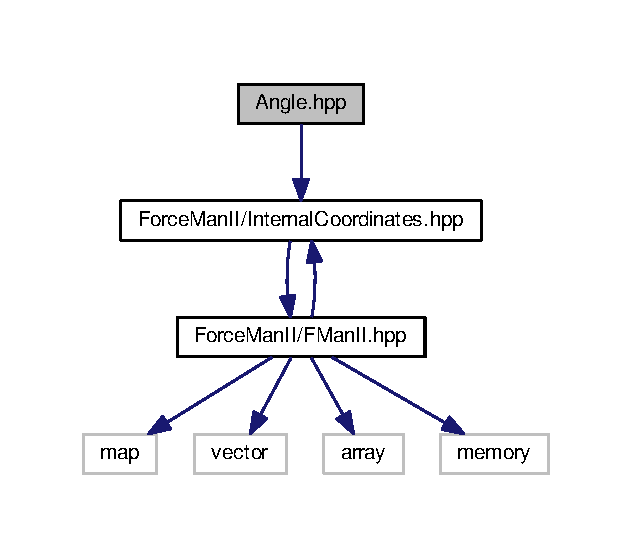
\includegraphics[width=304pt]{Angle_8hpp__incl}
\end{center}
\end{figure}
\subsection*{Classes}
\begin{DoxyCompactItemize}
\item 
class \hyperlink{classFManII_1_1Angle}{F\+Man\+I\+I\+::\+Angle}
\end{DoxyCompactItemize}
\subsection*{Namespaces}
\begin{DoxyCompactItemize}
\item 
 \hyperlink{namespaceFManII}{F\+Man\+II}
\begin{DoxyCompactList}\small\item\em Namespace for all code associated with Force\+Man\+II. \end{DoxyCompactList}\end{DoxyCompactItemize}


\subsection{Detailed Description}
\begin{DoxyVersion}{Version}
0.\+1 
\end{DoxyVersion}
\begin{DoxyDate}{Date}
October 29, 2016 at 12\+:55 PM (E\+ST)
\end{DoxyDate}
Original Author\+: \begin{DoxyAuthor}{Author}
Ryan M. Richard (ryanmrichard1$<$at$>$gmail.\+com)
\end{DoxyAuthor}
Additional contributions by\+: 
\hypertarget{Common_8hpp}{}\section{Common.\+hpp File Reference}
\label{Common_8hpp}\index{Common.\+hpp@{Common.\+hpp}}
{\ttfamily \#include $<$stdexcept$>$}\\*
{\ttfamily \#include $<$memory$>$}\\*
Include dependency graph for Common.\+hpp\+:\nopagebreak
\begin{figure}[H]
\begin{center}
\leavevmode
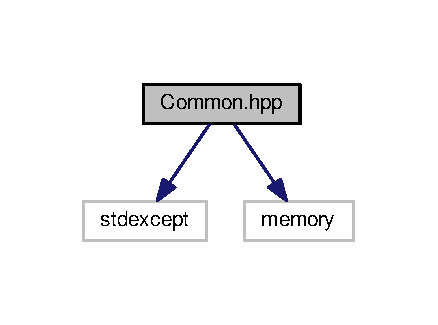
\includegraphics[width=210pt]{Common_8hpp__incl}
\end{center}
\end{figure}
\subsection*{Namespaces}
\begin{DoxyCompactItemize}
\item 
 \hyperlink{namespaceFManII}{F\+Man\+II}
\begin{DoxyCompactList}\small\item\em Namespace for all code associated with Force\+Man\+II. \end{DoxyCompactList}\end{DoxyCompactItemize}
\subsection*{Macros}
\begin{DoxyCompactItemize}
\item 
\#define {\bfseries D\+E\+B\+U\+G\+\_\+\+C\+H\+E\+CK}(cond,  msg)~do\{C\+H\+E\+CK(cond,msg);\}while(0)\hypertarget{Common_8hpp_a101d424293aea1b08114a8e56aebff1c}{}\label{Common_8hpp_a101d424293aea1b08114a8e56aebff1c}

\end{DoxyCompactItemize}
\subsection*{Functions}
\begin{DoxyCompactItemize}
\item 
{\footnotesize template$<$typename T , typename... Args$>$ }\\std\+::unique\+\_\+ptr$<$ T $>$ \hyperlink{namespaceFManII_a57e9a715666f24e78bd0025020e2c08e}{F\+Man\+I\+I\+::make\+\_\+unique} (Args \&\&...args)\hypertarget{namespaceFManII_a57e9a715666f24e78bd0025020e2c08e}{}\label{namespaceFManII_a57e9a715666f24e78bd0025020e2c08e}

\begin{DoxyCompactList}\small\item\em Once C++14 is accepted we can use std\+::make\+\_\+unique, till then we have this. \end{DoxyCompactList}\item 
void {\bfseries F\+Man\+I\+I\+::\+C\+H\+E\+CK} (bool cond, const std\+::string \&msg)\hypertarget{namespaceFManII_a70d1cfbb2f83f24521e0f0a31df25fd4}{}\label{namespaceFManII_a70d1cfbb2f83f24521e0f0a31df25fd4}

\end{DoxyCompactItemize}


\subsection{Detailed Description}
File containing common helper functions

\begin{DoxyVersion}{Version}
0.\+1 
\end{DoxyVersion}
\begin{DoxyDate}{Date}
October 1, 2016 at 1\+:23 PM (E\+ST)
\end{DoxyDate}
Original Author\+: \begin{DoxyAuthor}{Author}
Ryan M. Richard (ryanmrichard1$<$at$>$gmail.\+com)
\end{DoxyAuthor}
Additional contributions by\+: 
\hypertarget{Distance_8hpp}{}\section{Distance.\+hpp File Reference}
\label{Distance_8hpp}\index{Distance.\+hpp@{Distance.\+hpp}}
{\ttfamily \#include \char`\"{}Force\+Man\+I\+I/\+Internal\+Coordinates.\+hpp\char`\"{}}\\*
Include dependency graph for Distance.\+hpp\+:\nopagebreak
\begin{figure}[H]
\begin{center}
\leavevmode
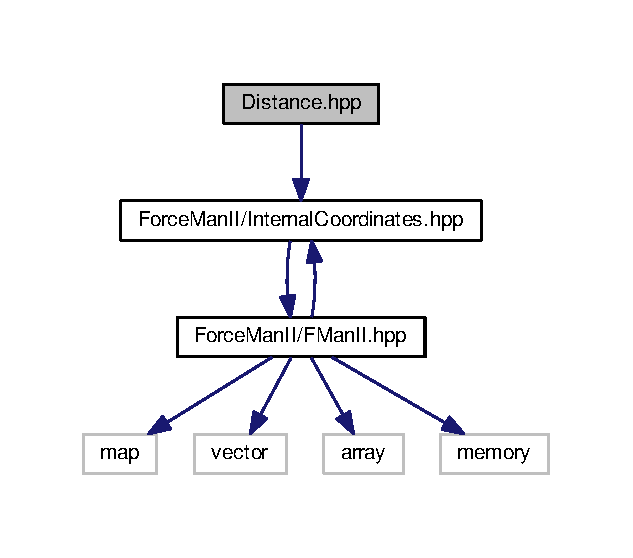
\includegraphics[width=304pt]{Distance_8hpp__incl}
\end{center}
\end{figure}
\subsection*{Classes}
\begin{DoxyCompactItemize}
\item 
class \hyperlink{classFManII_1_1Distance}{F\+Man\+I\+I\+::\+Distance}
\end{DoxyCompactItemize}
\subsection*{Namespaces}
\begin{DoxyCompactItemize}
\item 
 \hyperlink{namespaceFManII}{F\+Man\+II}
\begin{DoxyCompactList}\small\item\em Namespace for all code associated with Force\+Man\+II. \end{DoxyCompactList}\end{DoxyCompactItemize}


\subsection{Detailed Description}
\begin{DoxyVersion}{Version}
0.\+1 
\end{DoxyVersion}
\begin{DoxyDate}{Date}
October 9, 2016 at 12\+:51 PM (E\+ST)
\end{DoxyDate}
Original Author\+: \begin{DoxyAuthor}{Author}
Ryan M. Richard (ryanmrichard1$<$at$>$gmail.\+com)
\end{DoxyAuthor}
Additional contributions by\+: 
\hypertarget{FFTerm_8hpp}{}\section{F\+F\+Term.\+hpp File Reference}
\label{FFTerm_8hpp}\index{F\+F\+Term.\+hpp@{F\+F\+Term.\+hpp}}
\subsection*{Classes}
\begin{DoxyCompactItemize}
\item 
class \hyperlink{classFManII_1_1FFTerm}{F\+Man\+I\+I\+::\+F\+F\+Term$<$ Model\+\_\+t, Coord\+\_\+t $>$}
\end{DoxyCompactItemize}
\subsection*{Namespaces}
\begin{DoxyCompactItemize}
\item 
 \hyperlink{namespaceFManII}{F\+Man\+II}
\begin{DoxyCompactList}\small\item\em Namespace for all code associated with Force\+Man\+II. \end{DoxyCompactList}\end{DoxyCompactItemize}


\subsection{Detailed Description}
\begin{DoxyVersion}{Version}
0.\+1 
\end{DoxyVersion}
\begin{DoxyDate}{Date}
October 1, 2016 at 11\+:32 AM (E\+ST)
\end{DoxyDate}
Original Author\+: \begin{DoxyAuthor}{Author}
Ryan M. Richard (ryanmrichard1$<$at$>$gmail.\+com)
\end{DoxyAuthor}
Additional contributions by\+: 
\hypertarget{FManII_8hpp}{}\section{F\+Man\+I\+I.\+hpp File Reference}
\label{FManII_8hpp}\index{F\+Man\+I\+I.\+hpp@{F\+Man\+I\+I.\+hpp}}


This header is meant to be the main A\+PI to Force\+Man\+II. Anything users need to interface with Force\+Man\+II goes here.  


{\ttfamily \#include $<$map$>$}\\*
{\ttfamily \#include $<$vector$>$}\\*
{\ttfamily \#include $<$array$>$}\\*
{\ttfamily \#include $<$memory$>$}\\*
{\ttfamily \#include \char`\"{}Force\+Man\+I\+I/\+Internal\+Coordinates.\+hpp\char`\"{}}\\*
Include dependency graph for F\+Man\+I\+I.\+hpp\+:\nopagebreak
\begin{figure}[H]
\begin{center}
\leavevmode
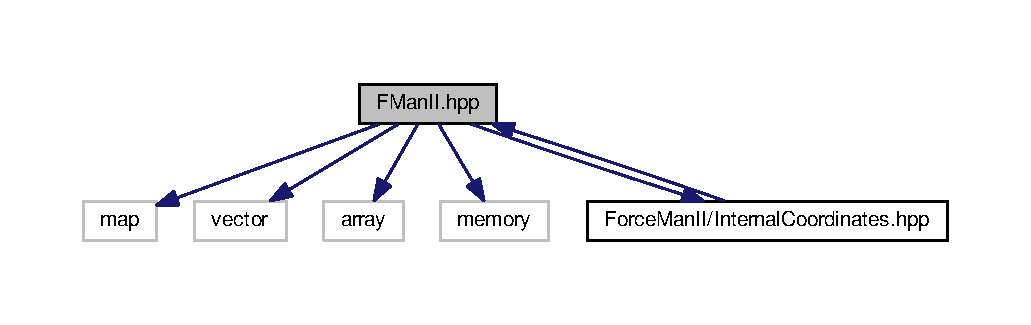
\includegraphics[width=350pt]{FManII_8hpp__incl}
\end{center}
\end{figure}
This graph shows which files directly or indirectly include this file\+:\nopagebreak
\begin{figure}[H]
\begin{center}
\leavevmode
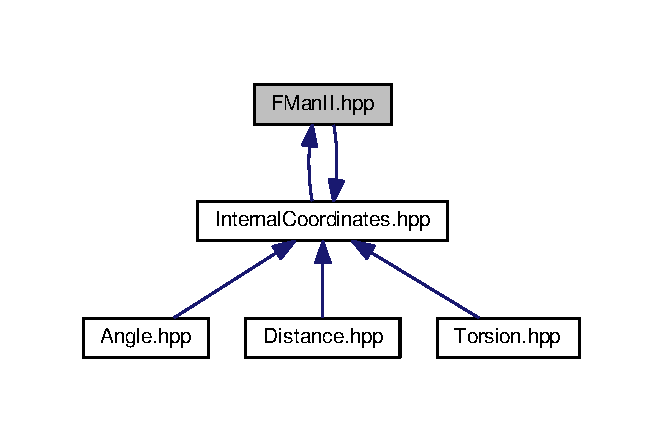
\includegraphics[width=318pt]{FManII_8hpp__dep__incl}
\end{center}
\end{figure}
\subsection*{Namespaces}
\begin{DoxyCompactItemize}
\item 
 \hyperlink{namespaceFManII}{F\+Man\+II}
\begin{DoxyCompactList}\small\item\em Namespace for all code associated with Force\+Man\+II. \end{DoxyCompactList}\end{DoxyCompactItemize}
\subsection*{Typedefs}
\begin{DoxyCompactItemize}
\item 
using \hyperlink{namespaceFManII_a988516dba14437f483faf9f3c6d40c25}{F\+Man\+I\+I\+::\+Coord\+Array} = std\+::map$<$ Int\+Coord\+\_\+t, std\+::unique\+\_\+ptr$<$ Int\+Coords $>$$>$\hypertarget{namespaceFManII_a988516dba14437f483faf9f3c6d40c25}{}\label{namespaceFManII_a988516dba14437f483faf9f3c6d40c25}

\begin{DoxyCompactList}\small\item\em An array of internal coordinates arranged by type. \end{DoxyCompactList}\item 
using \hyperlink{namespaceFManII_add1cccdf9425a71de6835b2631b84db8}{F\+Man\+I\+I\+::\+Atom\+Types} = std\+::vector$<$ std\+::array$<$ size\+\_\+t, 2 $>$$>$\hypertarget{namespaceFManII_add1cccdf9425a71de6835b2631b84db8}{}\label{namespaceFManII_add1cccdf9425a71de6835b2631b84db8}

\begin{DoxyCompactList}\small\item\em Array where element i respectively is the atom type and V\+DW type of atom i. \end{DoxyCompactList}\item 
using \hyperlink{namespaceFManII_a7c18a61f01fcc0604c39cbfae43665df}{F\+Man\+I\+I\+::\+Conn\+Data} = std\+::vector$<$ std\+::vector$<$ size\+\_\+t $>$$>$\hypertarget{namespaceFManII_a7c18a61f01fcc0604c39cbfae43665df}{}\label{namespaceFManII_a7c18a61f01fcc0604c39cbfae43665df}

\begin{DoxyCompactList}\small\item\em Array such that element i is a vector of the atoms bonded to atom i. \end{DoxyCompactList}\item 
using \hyperlink{namespaceFManII_a16edca665b5dfcdf9b3995844ad01bb5}{F\+Man\+I\+I\+::\+Param\+Types} = std\+::map$<$ Int\+Coord\+\_\+t, std\+::map$<$ Param\+\_\+t, std\+::map$<$ std\+::vector$<$ size\+\_\+t $>$, double $>$$>$$>$
\begin{DoxyCompactList}\small\item\em An object to hold the parameters of a force field. \end{DoxyCompactList}\end{DoxyCompactItemize}
\subsection*{Enumerations}
\begin{DoxyCompactItemize}
\item 
enum \hyperlink{namespaceFManII_ab331802fde4c5f2564443f1704c25363}{F\+Man\+I\+I\+::\+Param\+\_\+t} \{ \\*
\hyperlink{namespaceFManII_ab331802fde4c5f2564443f1704c25363acce4c4e3a7008d8a210e0950f0ae6646}{F\+Man\+I\+I\+::K}, 
\hyperlink{namespaceFManII_ab331802fde4c5f2564443f1704c25363adbd624e837d07235c15569341fa0c052}{F\+Man\+I\+I\+::r0}, 
\hyperlink{namespaceFManII_ab331802fde4c5f2564443f1704c25363a807f5303050e210f41b43189457ee216}{F\+Man\+I\+I\+::amp}, 
\hyperlink{namespaceFManII_ab331802fde4c5f2564443f1704c25363a3a18cc339dcc327297994fd5de406000}{F\+Man\+I\+I\+::phi}, 
\\*
\hyperlink{namespaceFManII_ab331802fde4c5f2564443f1704c25363a351f38f2149aa0e3be56f7c5aa16eae9}{F\+Man\+I\+I\+::n}, 
\hyperlink{namespaceFManII_ab331802fde4c5f2564443f1704c25363a6168b053bb4d250bc56878c3c5329606}{F\+Man\+I\+I\+::amp2}, 
\hyperlink{namespaceFManII_ab331802fde4c5f2564443f1704c25363ac923a156e5d6c899b0691bcf05dbfe08}{F\+Man\+I\+I\+::phi2}, 
\hyperlink{namespaceFManII_ab331802fde4c5f2564443f1704c25363a79574f7c7d028868bba201ab99eeb319}{F\+Man\+I\+I\+::n2}, 
\\*
\hyperlink{namespaceFManII_ab331802fde4c5f2564443f1704c25363a8ea674fa14845cb499bba588e8e6b72d}{F\+Man\+I\+I\+::amp3}, 
\hyperlink{namespaceFManII_ab331802fde4c5f2564443f1704c25363a48029f18757fa6d2a3d72517001cc0d1}{F\+Man\+I\+I\+::phi3}, 
\hyperlink{namespaceFManII_ab331802fde4c5f2564443f1704c25363ac582c34207ea213912ced08cebca1a34}{F\+Man\+I\+I\+::n3}, 
\hyperlink{namespaceFManII_ab331802fde4c5f2564443f1704c25363afec764e5c20f480b9b706861106356de}{F\+Man\+I\+I\+::q}, 
\\*
\hyperlink{namespaceFManII_ab331802fde4c5f2564443f1704c25363a0cdd92becbae953906c5305392e29836}{F\+Man\+I\+I\+::sigma}, 
\hyperlink{namespaceFManII_ab331802fde4c5f2564443f1704c25363a59874bb4d679327306f2c7405286afa9}{F\+Man\+I\+I\+::epsilon}
 \}\begin{DoxyCompactList}\small\item\em These are the recognized types of parameters. \end{DoxyCompactList}
\item 
enum \hyperlink{namespaceFManII_aee2b0c5668a8970ffb58ac650994e059}{F\+Man\+I\+I\+::\+Int\+Coord\+\_\+t} \{ \\*
\hyperlink{namespaceFManII_aee2b0c5668a8970ffb58ac650994e059a0ad48919334546233ad86a2699918852}{F\+Man\+I\+I\+::\+B\+O\+ND}, 
\hyperlink{namespaceFManII_aee2b0c5668a8970ffb58ac650994e059ae3fda21c728a90c9974bb2a2404efcc7}{F\+Man\+I\+I\+::\+U\+B\+P\+A\+IR}, 
\hyperlink{namespaceFManII_aee2b0c5668a8970ffb58ac650994e059ad387432e20772e11fb6520606b93faa6}{F\+Man\+I\+I\+::\+P\+A\+IR}, 
\hyperlink{namespaceFManII_aee2b0c5668a8970ffb58ac650994e059ad67623636070f3be7ae6e7700a5bd9f6}{F\+Man\+I\+I\+::\+A\+N\+G\+LE}, 
\\*
\hyperlink{namespaceFManII_aee2b0c5668a8970ffb58ac650994e059a4f481d454dea70e1a1c7ef63d99d3402}{F\+Man\+I\+I\+::\+T\+O\+R\+S\+I\+ON}, 
\hyperlink{namespaceFManII_aee2b0c5668a8970ffb58ac650994e059a650ab62f01654d8aae5b3a9c9919dbed}{F\+Man\+I\+I\+::\+I\+M\+P\+T\+O\+R\+S\+I\+ON}, 
\hyperlink{namespaceFManII_aee2b0c5668a8970ffb58ac650994e059af32be9c7ba6cd66722cc93629dbb5fbe}{F\+Man\+I\+I\+::\+E\+L\+E\+C\+T\+R\+O\+S\+T\+A\+T\+I\+CS}, 
\hyperlink{namespaceFManII_aee2b0c5668a8970ffb58ac650994e059a97b415b3364dd5c1da0fd17a551ce037}{F\+Man\+I\+I\+::\+L\+E\+N\+N\+A\+R\+D\+\_\+\+J\+O\+N\+ES}
 \}\begin{DoxyCompactList}\small\item\em These are the recognized types of Int\+Coords. \end{DoxyCompactList}
\end{DoxyCompactItemize}
\subsection*{Functions}
\begin{DoxyCompactItemize}
\item 
Coord\+Array \hyperlink{namespaceFManII_a962553cf7a05889bf0f90071a59d963c}{F\+Man\+I\+I\+::get\+\_\+coords} (const std\+::vector$<$ double $>$ \&Carts, const Atom\+Types \&Types, const Param\+Types \&Params, const Conn\+Data \&Conns, double chg14scale=1.\+0)
\begin{DoxyCompactList}\small\item\em A function that processes the input and returns a set of objects set up for use in \hyperlink{namespaceFManII}{F\+Man\+II}. \end{DoxyCompactList}\end{DoxyCompactItemize}


\subsection{Detailed Description}
\begin{DoxyVersion}{Version}
0.\+1 
\end{DoxyVersion}
\begin{DoxyDate}{Date}
October 14, 2016 at 10\+:17 PM (E\+ST)
\end{DoxyDate}
Original Author\+: \begin{DoxyAuthor}{Author}
Ryan M. Richard (ryanmrichard1$<$at$>$gmail.\+com)
\end{DoxyAuthor}
Additional contributions by\+: 
\hypertarget{FourierSeries_8hpp}{}\section{Fourier\+Series.\+hpp File Reference}
\label{FourierSeries_8hpp}\index{Fourier\+Series.\+hpp@{Fourier\+Series.\+hpp}}
{\ttfamily \#include $<$vector$>$}\\*
Include dependency graph for Fourier\+Series.\+hpp\+:\nopagebreak
\begin{figure}[H]
\begin{center}
\leavevmode
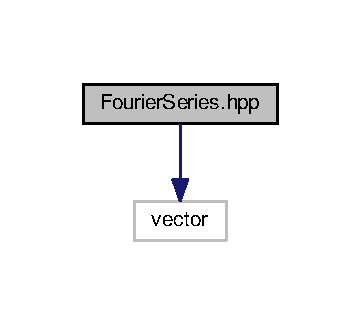
\includegraphics[width=173pt]{FourierSeries_8hpp__incl}
\end{center}
\end{figure}
\subsection*{Classes}
\begin{DoxyCompactItemize}
\item 
struct \hyperlink{structFManII_1_1FourierSeries}{F\+Man\+I\+I\+::\+Fourier\+Series}
\begin{DoxyCompactList}\small\item\em Implements a Fourier Series model potential. \end{DoxyCompactList}\end{DoxyCompactItemize}
\subsection*{Namespaces}
\begin{DoxyCompactItemize}
\item 
 \hyperlink{namespaceFManII}{F\+Man\+II}
\begin{DoxyCompactList}\small\item\em Namespace for all code associated with Force\+Man\+II. \end{DoxyCompactList}\end{DoxyCompactItemize}


\subsection{Detailed Description}
\begin{DoxyVersion}{Version}
0.\+1 
\end{DoxyVersion}
\begin{DoxyDate}{Date}
November 19, 2016 at 2\+:09 PM (E\+ST)
\end{DoxyDate}
Original Author\+: \begin{DoxyAuthor}{Author}
Ryan M. Richard (ryanmrichard1$<$at$>$gmail.\+com)
\end{DoxyAuthor}
Additional contributions by\+: 
\hypertarget{HarmonicOscillator_8hpp}{}\section{Harmonic\+Oscillator.\+hpp File Reference}
\label{HarmonicOscillator_8hpp}\index{Harmonic\+Oscillator.\+hpp@{Harmonic\+Oscillator.\+hpp}}
{\ttfamily \#include $<$vector$>$}\\*
Include dependency graph for Harmonic\+Oscillator.\+hpp\+:\nopagebreak
\begin{figure}[H]
\begin{center}
\leavevmode
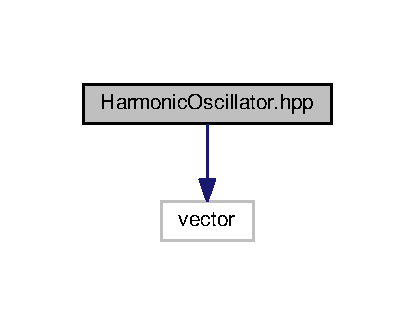
\includegraphics[width=199pt]{HarmonicOscillator_8hpp__incl}
\end{center}
\end{figure}
\subsection*{Classes}
\begin{DoxyCompactItemize}
\item 
struct \hyperlink{structFManII_1_1HarmonicOscillator}{F\+Man\+I\+I\+::\+Harmonic\+Oscillator}
\begin{DoxyCompactList}\small\item\em Implements the harmonic oscillator model potential. \end{DoxyCompactList}\end{DoxyCompactItemize}
\subsection*{Namespaces}
\begin{DoxyCompactItemize}
\item 
 \hyperlink{namespaceFManII}{F\+Man\+II}
\begin{DoxyCompactList}\small\item\em Namespace for all code associated with Force\+Man\+II. \end{DoxyCompactList}\end{DoxyCompactItemize}


\subsection{Detailed Description}
\begin{DoxyVersion}{Version}
0.\+1 
\end{DoxyVersion}
\begin{DoxyDate}{Date}
October 1, 2016 at 12\+:33 PM (E\+ST)
\end{DoxyDate}
Original Author\+: \begin{DoxyAuthor}{Author}
Ryan M. Richard (ryanmrichard1$<$at$>$gmail.\+com)
\end{DoxyAuthor}
Additional contributions by\+: 
\hypertarget{Torsion_8hpp}{}\section{Torsion.\+hpp File Reference}
\label{Torsion_8hpp}\index{Torsion.\+hpp@{Torsion.\+hpp}}
{\ttfamily \#include \char`\"{}Force\+Man\+I\+I/\+Internal\+Coordinates.\+hpp\char`\"{}}\\*
Include dependency graph for Torsion.\+hpp\+:\nopagebreak
\begin{figure}[H]
\begin{center}
\leavevmode
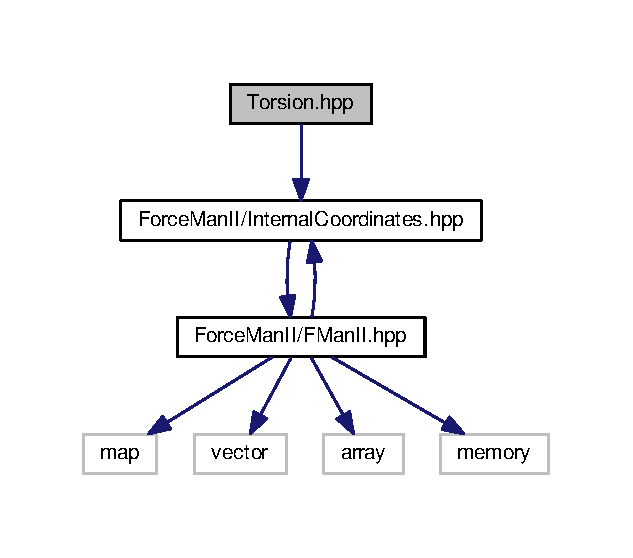
\includegraphics[width=304pt]{Torsion_8hpp__incl}
\end{center}
\end{figure}
\subsection*{Classes}
\begin{DoxyCompactItemize}
\item 
class \hyperlink{classFManII_1_1Torsion}{F\+Man\+I\+I\+::\+Torsion}
\end{DoxyCompactItemize}
\subsection*{Namespaces}
\begin{DoxyCompactItemize}
\item 
 \hyperlink{namespaceFManII}{F\+Man\+II}
\begin{DoxyCompactList}\small\item\em Namespace for all code associated with Force\+Man\+II. \end{DoxyCompactList}\end{DoxyCompactItemize}


\subsection{Detailed Description}
\begin{DoxyVersion}{Version}
0.\+1 
\end{DoxyVersion}
\begin{DoxyDate}{Date}
November 6, 2016 at 1\+:21 PM (E\+ST)
\end{DoxyDate}
Original Author\+: \begin{DoxyAuthor}{Author}
Ryan M. Richard (ryanmrichard1$<$at$>$gmail.\+com)
\end{DoxyAuthor}
Additional contributions by\+: 
\hypertarget{Util_8hpp}{}\section{Util.\+hpp File Reference}
\label{Util_8hpp}\index{Util.\+hpp@{Util.\+hpp}}
{\ttfamily \#include $<$array$>$}\\*
{\ttfamily \#include $<$numeric$>$}\\*
{\ttfamily \#include $<$cmath$>$}\\*
Include dependency graph for Util.\+hpp\+:\nopagebreak
\begin{figure}[H]
\begin{center}
\leavevmode
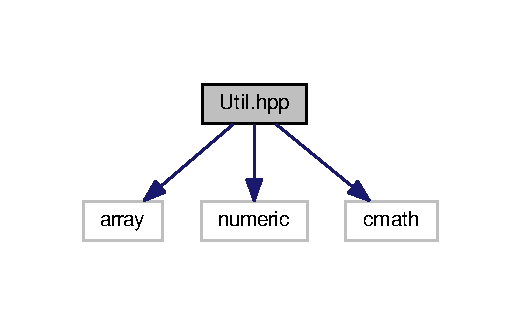
\includegraphics[width=250pt]{Util_8hpp__incl}
\end{center}
\end{figure}
\subsection*{Namespaces}
\begin{DoxyCompactItemize}
\item 
 \hyperlink{namespaceFManII}{F\+Man\+II}
\begin{DoxyCompactList}\small\item\em Namespace for all code associated with Force\+Man\+II. \end{DoxyCompactList}\end{DoxyCompactItemize}
\subsection*{Functions}
\begin{DoxyCompactItemize}
\item 
{\footnotesize template$<$typename T $>$ }\\std\+::array$<$ double, 3 $>$ \hyperlink{namespaceFManII_ab6c3ba0221d1479590c328071add3a69}{F\+Man\+I\+I\+::cross} (const T \&v1, const T \&v2)\hypertarget{namespaceFManII_ab6c3ba0221d1479590c328071add3a69}{}\label{namespaceFManII_ab6c3ba0221d1479590c328071add3a69}

\begin{DoxyCompactList}\small\item\em Returns the cross product of two vectors. \end{DoxyCompactList}\item 
{\footnotesize template$<$typename T $>$ }\\std\+::array$<$ double, 3 $>$ \hyperlink{namespaceFManII_a67d2288b51cdc78b0569812bbbe7603c}{F\+Man\+I\+I\+::diff} (const T \&v1, const T \&v2)\hypertarget{namespaceFManII_a67d2288b51cdc78b0569812bbbe7603c}{}\label{namespaceFManII_a67d2288b51cdc78b0569812bbbe7603c}

\begin{DoxyCompactList}\small\item\em Returns the difference between two vectors, v1-\/v2. \end{DoxyCompactList}\item 
double \hyperlink{namespaceFManII_a804811720c4566ddd330e4abc8d2c65f}{F\+Man\+I\+I\+::dot} (const std\+::array$<$ double, 3 $>$ \&v1, const std\+::array$<$ double, 3 $>$ \&v2)\hypertarget{namespaceFManII_a804811720c4566ddd330e4abc8d2c65f}{}\label{namespaceFManII_a804811720c4566ddd330e4abc8d2c65f}

\begin{DoxyCompactList}\small\item\em Returns the dot product of two vectors. \end{DoxyCompactList}\item 
double \hyperlink{namespaceFManII_a88126c99fc2140b9a3c37d695337fd6a}{F\+Man\+I\+I\+::mag} (const std\+::array$<$ double, 3 $>$ \&v1)\hypertarget{namespaceFManII_a88126c99fc2140b9a3c37d695337fd6a}{}\label{namespaceFManII_a88126c99fc2140b9a3c37d695337fd6a}

\begin{DoxyCompactList}\small\item\em Returns the magnitude of a vector. \end{DoxyCompactList}\item 
double \hyperlink{namespaceFManII_a45ace6891d8e67f7e4b679300533e0ac}{F\+Man\+I\+I\+::angle} (const std\+::array$<$ double, 3 $>$ \&v1, const std\+::array$<$ double, 3 $>$ \&v2, const std\+::array$<$ double, 3 $>$ \&n)
\end{DoxyCompactItemize}


\subsection{Detailed Description}
Contains helper utility functions of a mathematical nature

\begin{DoxyVersion}{Version}
0.\+1 
\end{DoxyVersion}
\begin{DoxyDate}{Date}
November 6, 2016 at 1\+:38 PM (E\+ST)
\end{DoxyDate}
Original Author\+: \begin{DoxyAuthor}{Author}
Ryan M. Richard (ryanmrichard1$<$at$>$gmail.\+com)
\end{DoxyAuthor}
Additional contributions by\+: 
%--- End generated contents ---

% Index
\backmatter
\newpage
\phantomsection
\clearemptydoublepage
\addcontentsline{toc}{chapter}{Index}
\printindex

\end{document}
